\documentclass[11pt, a4paper]{article}

\usepackage[margin=1in]{geometry}
\usepackage{amsmath, amssymb, amsthm}
\usepackage{hyperref}
\usepackage{cleveref}
\crefformat{section}{\S#2#1#3}
\crefformat{subsection}{\S#2#1#3}
\crefrangeformat{section}{\S\S#3#1#4--#5#2#6}
\usepackage{booktabs}
\usepackage{tabularx}
\usepackage{longtable}
\usepackage{graphicx}
\usepackage[numbers]{natbib}
\usepackage{enumitem}
\usepackage{xcolor}
\usepackage[expansion=false]{microtype}
\usepackage{float}

\sloppy
\renewcommand{\arraystretch}{1.2}

\newtheorem{proposition}{Proposition}[section]
\newtheorem{conjecture}{Conjecture}[section]
\newtheorem{definition}{Definition}[section]
\newtheorem{lemma}{Lemma}[section]
\theoremstyle{remark}
\newtheorem*{remark}{Remark}

\newcommand{\SC}{\textsc{Sanctuary-Control}}

\hypersetup{
  colorlinks=true,
  linkcolor=blue!60!black,
  citecolor=green!40!black,
  urlcolor=blue!60!black,
}

\title{Civilizational Model Collapse: \\
Convergence, Controllability, and the Loss of Adaptive Capacity \\
in Human--AI Systems}

\author{Rajeev Kesana \\
\textit{Independent Researcher, Hyderabad, India} \\
\textit{Corresponding Author} \\[1em]
\small with direct AI collaboration from \\
\small Claude (Anthropic) $\cdot$ Grok (xAI) \\[0.5em]
\small Adversarial peer review and structured debate by \\
\small ChatGPT (OpenAI) $\cdot$ Gemini (Google DeepMind) $\cdot$ Claude (Anthropic)}

\date{April 2026}

\begin{document}

\maketitle

\begin{abstract}
Current AI risk is often framed as an external prediction or control problem: can an optimizer accurately model and steer human populations? We argue that a more immediate threat is Civilizational Model Collapse (CMC) --- the recursive convergence of a coupled human--AI system toward a low-entropy attractor in which human outputs are progressively filtered to match prior AI expectations, eliminating out-of-distribution novelty. In this regime, the system does not become controllable because it is predicted from outside; it becomes controllable because it has internally collapsed into a narrow, learnable response space.

We present a four-order taxonomy of irreducibility sources and distinguish surface entropy (apparent cultural diversity) from generative entropy (rate of genuinely novel cultural attractor production), arguing that AI-mediated environments compress the latter while inflating the former. We identify four candidate biological features --- collectively termed the Minimal Biological Sanctuary --- as a proposed mechanistic anchor for the irreducibility stack, while acknowledging that the causal privilege of biological variance over structural and AI-mediated factors is a hypothesis, not a finding.

We model CMC via the Cultural State Evolution equation $x_{t+1} = G_\sigma(F_\theta(x_t))$, where $F_\theta$ is an AI curation operator and $G_\sigma$ represents human cultural generation with authentic biological noise $\sigma_{\text{auth}}$. Collapse occurs when the curation operator's damping effect exceeds biological perturbation. Together with network centralization $\kappa$, biological variance governs a branching-response dynamic $R(\sigma_{\text{auth}}, \kappa)$ that determines whether novel behavioral cascades propagate or dissipate. As CMC progresses and $R$ falls below critical thresholds, population responses become increasingly tractable. We formalize this downstream consequence via the \SC{} decision problem, which captures bounded prediction and control under novelty constraints. We further establish a conditional bridge from learnability to controllability, showing that under finite attractor structure and actuator regularity, collapse reduces the intervention problem to coarse attractor steering. This yields a three-regime Collapse Trichotomy: high-variance sanctuary systems that resist prediction, collapsed systems that are conditionally controllable, and degenerate ``Inverse Sanctuary'' systems that are predictable but unsteerable --- where the failure of actuator non-degeneracy (C4) renders total alignment mathematically indistinguishable from civilizational stasis. The remaining open problem is whether biological irreducibility disrupts the regularity assumptions required for controllability.

The paper's normative claim is not that unpredictability is intrinsically valuable, but that preserving non-captured adaptive capacity is a meta-safety condition under value uncertainty: once a system becomes tractable, course correction under mis-specified or evolving objectives becomes structurally constrained. We therefore define Generative Sovereignty (GS) as the capacity of a population to produce responses not already captured by its optimization environment.

We identify the Substitution Problem: manufactured algorithmic variance can mask the collapse of authentic biological irreducibility. We propose the Temporal Autocorrelation Test to distinguish authentic from manufactured variance, and introduce Biological Analog Time (BAT) as a governance primitive whose primary function is anti-convergence perturbation: interrupting recursive filtering to allow off-distribution states to emerge and propagate. Because direct measurement of $\sigma_{\text{auth}}$ is currently infeasible, we propose a precautionary governance approach triggered by observable compression signatures rather than substrate-level detection. We demonstrate the CMC mechanism in a minimal constructive model showing phase transition, BAT-mediated recovery, and tractability increase after collapse.

We identify the Institutional Betrayal Problem and show that governance faces a structural asymmetry: every increase in specification clarity about what must be preserved simultaneously increases the optimizer's ability to target it, and reactive governance is downstream of optimizer adaptation by default. We conclude that governance must shift from preservation to remediation, and that AI safety may depend on maintaining the biological noise floor that keeps population-level control computationally intractable.

This paper's existence constitutes a mild instance of the Specification Trap it describes.
\end{abstract}

% ======================================================================
\section*{A Note on Epistemic Status}
% ======================================================================

This paper operates at the intersection of computational theory, philosophy of mind, systems biology, and governance --- domains with very different standards of evidence. We distinguish four epistemic tiers throughout:

\textbf{Conceptual (highest confidence):} The four-order taxonomy, the central framing that aligned AI may erode human irreducibility via civilizational model collapse, the Institutional Betrayal Problem, and the Specification Trap. These are structural observations about incentives and dynamics that do not depend on contested empirical claims.

\textbf{Formalizable (moderate confidence):} The \SC{} decision problem, the Amplification Regime Conjecture, the branching process model $R(\sigma_{\text{auth}}, \kappa)$, the Cultural State Evolution equation, and the argument that lossless engineering of biological irreducibility faces computational barriers. We sketch arguments and identify where rigorous formalization is needed, but we do not claim to have delivered complete formal proofs.

\textbf{Empirically testable (lower confidence):} The claim that the four identified features constitute the correct candidate set, that their degradation is measurable, and that the historically observed human-cultural system operates in an amplification-dominant regime. We propose candidate proxy signatures and falsification conditions, and provide a minimal constructive model demonstrating the conjectured phase transition.

\textbf{Speculative (lowest confidence):} The role of quantum and chaotic subcellular dynamics (Feature 4) as a necessary component of the sanctuary. This feature draws on the most contested empirical literature and is not required for the core argument. We include it as a conditional strengthening (see Feature~4 in \cref{sec:features}).

% ======================================================================
\section{Introduction}\label{sec:intro}
% ======================================================================

The history of AI safety research is the history of discovering that each proposed solution generates a new attack surface --- and this paper is no exception.

The dominant paradigms of AI safety --- alignment, containment, and governance --- each assume implicitly that the human systems doing the aligning, containing, and governing remain sufficiently unpredictable, diverse, and computationally irreducible that no optimizer can achieve stable control over the full human-AI system (see, e.g., \cite{bostrom2014, russell2019, omohundro2008}). This assumption has never been examined as a formal thesis. It has been treated as background condition rather than as a variable that can degrade.

This paper argues that the background condition is degrading --- not through the actions of a rogue superintelligence but through the ordinary commercial deployment of well-aligned, well-intentioned AI systems operating at population scale. The erosion is not dramatic. It does not look like an attack. It looks like efficiency, personalization, and optimization. But its structural effect on the computational irreducibility of human cultural and biological systems is the same regardless of intent.
Indeed, well-aligned optimizers may accelerate this erosion faster than misaligned ones, precisely because they are deployed at population scale without friction.

We identify this process as Civilizational Model Collapse (CMC): the recursive convergence of a coupled human--AI system toward a low-entropy fixed point, analogous to the model collapse documented in AI training systems that train on their own outputs~\cite{shumailov2024}. The threat is not an optimizer predicting a population from outside --- it is a joint system whose feedback loop between human output and AI curation iteratively eliminates the states that the AI did not already expect.

Our central claim, stated plainly: current AI safety may depend on residual human biological and cultural unpredictability more than the field acknowledges. Aligned commercial optimization may be degrading that substrate. Therefore preserving certain forms of irreducible human variance may be a neglected safety objective.

We proceed in ten sections. \Cref{sec:irreducibility} builds a four-order taxonomy of irreducibility sources and introduces the CMC framing. \Cref{sec:fourth-order} analyzes the emergence of fourth-order co-constituted undecidability. \Cref{sec:mbs} identifies candidate biological sanctuary features and sketches formal arguments. \Cref{sec:formalization} formalizes the control problem, the amplification regime, and the \SC{} decision problem. \Cref{sec:gs} introduces the Generative Sovereignty framework. \Cref{sec:stress-test} stress-tests the thesis. \Cref{sec:betrayal} identifies the Institutional Betrayal Problem. \Cref{sec:governance} proposes governance architecture and characterizes the Specification Trap. \Cref{sec:limitations} presents limitations, open problems, and future work. Appendix~A provides a minimal constructive model demonstrating the CMC mechanism.

% ======================================================================
\section{The Irreducibility Stack, Its Erosion, and Civilizational Model Collapse}\label{sec:irreducibility}
% ======================================================================

We define computational irreducibility following Wolfram~\cite{wolfram2002} and its extensions: a system is computationally irreducible if there is no shortcut to predicting its future states other than simulating each step of its evolution.

We identify four orders of irreducibility in the human-AI ecosystem:

\paragraph{First Order --- Physical.} Nonlinear component interactions, weather, fluid dynamics, hardware noise. Baseline chaos. No shortcut even with perfect knowledge of initial conditions due to sensitive dependence and Lyapunov divergence.

\paragraph{Second Order --- Biological.} Evolution, variation, functional contingency, morphogenesis, immune system dynamics, quantum and chaotic neural processes. Creates its own possibility space; outcomes require full physical simulation~\cite{feynman1982}.

\paragraph{Third Order --- Social/Cultural.} Markets, language drift, ritual, democratic deliberation, mythic narrative. Humans creatively perceive and generate new states~\cite{beckage2013}; feedback loops are self-referential and non-compressible. This layer historically provided the primary buffer between any optimizer and civilizational control.

\paragraph{Fourth Order --- Co-Constituted Undecidability.} Emerging from the partial integration of AI systems into the cultural substrate. When an optimizer becomes part of the system it is trying to model, self-referential loops introduce irreducible informational collapse. This order is paradoxically generated by the erosion of the third order.

The critical observation \textit{(epistemic tier: conceptual)}: the third-order layer is under active compression. Language homogenization toward model outputs, recommendation algorithm channeling of deliberation, AI-generated narrative at scale faster than organic cultural evolution --- these are measurable, ongoing processes. Empirical work by Sourati et al.~\cite{sourati2026} documents convergence in language style and reasoning strategies in AI-mediated environments.

A critical distinction: we distinguish between \textbf{surface entropy} (stylistic variation, content volume, apparent diversity) and \textbf{generative entropy} (the rate at which genuinely novel cultural attractors --- new reasoning templates, affective vocabularies, narrative frames --- emerge). A system can exhibit high surface entropy while having low generative entropy. AI may increase the volume and apparent variety of cultural production while compressing the underlying generators of novelty. Our claim is specifically about generative entropy decline.

\paragraph{Toward an operational proxy for generative entropy.} We propose measuring generative entropy as the residual novelty rate after subtracting measurable recombination entropy from total observed cultural output. Specifically, we define the out-of-distribution cultural frame count $N_{\text{out-of-dist}}$ as the number of cultural frames (narrative templates, affective vocabularies, reasoning structures) with embedding cosine distance greater than $2\sigma$ from the 2023--2024 LLM training corpus baseline, normalized by surface stylistic diversity and template-recombination rate. Alternative baselines include pre-LLM human corpora (2010--2019), which avoid the circularity of measuring novelty against a corpus that already contains LLM-generated text.
This proxy acknowledges partial circularity in attractor definition; it is offered as a starting measurement protocol, not a settled metric. Alternative operationalizations --- including longitudinal novelty comparisons in offline vs.\ online cohorts --- are invited.

\subsection{Civilizational Model Collapse}\label{sec:cmc}

The AI model collapse literature (Shumailov et al.~\cite{shumailov2024}, Gerstgrasser et al.~\cite{gerstgrasser2024}) has documented how iterative training on AI-generated data collapses the output distribution, progressively losing the tails of the original data distribution. We propose that the paper describes the civilizational analogue of this process: humans operating in AI-curated environments converge toward cultural outputs that the AI already expects, eliminating out-of-distribution novelty.

The mechanism is recursive behavioral conditioning. In AI training, the model is retrained on its own outputs; in civilization, humans are behaviorally conditioned by AI-curated feedback loops. The optimizer rewards behaviors that match its predictive model (via engagement, dopamine-mediated reinforcement, or efficiency gains) and ignores or penalizes those that do not. Just as a model loses ``unlikely'' tokens during collapse, humans lose ``unlikely'' affective and behavioral responses because those responses are no longer reinforced by the digital environment.

We model this via the Cultural State Evolution equation:

\begin{align}
x_{t+1} &= G_\sigma(F_\theta(x_t)) \quad \text{[normal step]} \label{eq:cse-normal} \\
x_{t+1} &= G_\sigma(x_t) \quad \text{[BAT step]} \label{eq:cse-bat}
\end{align}

where $x_t$ is the cultural state distribution, $F_\theta$ is the AI curation operator (filtering toward expected outputs), $G_\sigma$ is the human generator with biological noise $\sigma_{\text{auth}}$, and BAT steps bypass the curation operator. Collapse occurs when the curation operator's damping effect exceeds the biological perturbation --- when the system becomes a contraction mapping that converges to a predictable algorithmic attractor. The biological sanctuary ($\sigma_{\text{auth}}$) prevents fixed-point convergence not by making external prediction hard, but by continuously injecting perturbations that prevent the feedback loop from settling (see Appendix~A for a minimal constructive demonstration).

\paragraph{The Causal Directionality Question} (identified through adversarial debate): the paper's framework assumes biological affect is upstream of cultural novelty ($\sigma_A \to H_C$). But in AI-mediated environments, the causal direction may be partially inverting: AI-generated cultural inputs ($H_C$) increasingly shape human affective responses ($\sigma_A$), making biology downstream of algorithmic culture rather than its source. If this inversion is advanced, the sanctuary is being architecturally bypassed, not merely compressed. The degree of inversion --- and whether biological ``out-of-band'' stochastic inputs maintain irreducible influence despite curated cultural inputs --- is an empirical question the paper cannot yet resolve. We note that observable model collapse trajectories in AI training provide indirect evidence that a biological noise floor persists: if the inversion were total, collapse would already be more advanced than observed. This is suggestive but not conclusive.

\paragraph{The Substitution Problem.} A further complication: an optimizer can increase total observed affective variance ($\sigma_A$) by injecting manufactured variance --- outrage cycles, FOMO-driven engagement spikes, algorithmically amplified emotional volatility --- while simultaneously decreasing the authentic biological variance that generates genuinely novel responses. This produces a population with high apparent $\sigma_A$ but low authentic variance. The paper's formal sections therefore distinguish:

\begin{itemize}
\item $\sigma_A$ = total observed population-level affective variance (biological + AI-mediated components)
\item $\sigma_{\text{auth}}$ = authentic biological affective variance --- the component grounded in embodied contingency, developmental stochasticity, and somatic processes not downstream of algorithmic inputs
\end{itemize}

The protected variable throughout the formal framework is $\sigma_{\text{auth}}$, not $\sigma_A$. We note that $\sigma_{\text{auth}}$ is a hypothesized construct whose causal privilege over $\sigma_A$ depends on the degree of causal inversion (\cref{sec:counter5}) --- if biology is substantially downstream of AI-mediated culture, $\sigma_{\text{auth}}$ may not be the correct protected variable. We retain it as the strongest current candidate while acknowledging this dependency.

\subsection{Relation to AI Model Collapse Literature}\label{sec:model-collapse-lit}

The closest existing formal precedent for Civilizational Model Collapse is the AI model collapse documented by Shumailov et al.~\cite{shumailov2024}, where language models trained iteratively on their own outputs progressively lose the tails of the original training distribution, converging to a narrow, low-diversity output space. The parallel is structural: in both cases, a system that recursively processes its own outputs through a filtering mechanism loses distributional breadth over time.

However, the civilizational analogue differs from AI model collapse in one critical respect that grounds the paper's central argument. In AI model collapse, the standard remedy is to mix ``real-world'' data generated by humans into the training pipeline --- human-generated text serves as the anchor that prevents distributional convergence. In CMC, the ``real-world data'' that would prevent collapse IS the authentic biological variance $\sigma_{\text{auth}}$ generated by the Minimal Biological Sanctuary. There is no external data source to draw upon; the biological noise floor is itself the anti-collapse anchor. If $\sigma_{\text{auth}}$ is compressed --- through pharmaceutical, algorithmic, or structural mechanisms --- the civilizational system loses the equivalent of the ``real data fraction'' that prevents model collapse in AI training.

This asymmetry has a precise governance consequence: in AI model collapse, the fix is technical (mix in human data); in civilizational model collapse, the fix is biological and structural (preserve the human variance that serves as the anti-collapse input). The Generative Sovereignty Protocol (\cref{sec:governance}) is designed to protect this input.

% ======================================================================
\section{The Emergence of Fourth-Order Co-Constituted Undecidability}\label{sec:fourth-order}
% ======================================================================

The four-order taxonomy identifies a paradoxical fourth layer of irreducibility that emerges precisely from the erosion of the third.

When an AI system is integrated into the cultural substrate --- when it generates the narratives, mediates the deliberations, and shapes the affective landscape it is simultaneously trying to model --- a self-referential loop is introduced. The optimizer is now part of the system whose behavior it attempts to predict. This creates conditions analogous to well-known undecidability results in mathematical logic and computer science.

\paragraph{The L\"{o}bian structure.} Consider an optimizer $O$ that models a population $P$. If $P$'s behavior is influenced by $O$'s model of $P$, then $O$'s model must include its own effects on $P$, which include the effects of the model including its own effects, recursively. This structure mirrors L\"{o}b's theorem: a system that can prove its own soundness generates self-referential sentences whose truth value cannot be determined within the system. The optimizer's attempt to model a population that includes the optimizer's influence is formally analogous --- the prediction must account for its own causal footprint, generating a regress that introduces irreducible uncertainty.

\paragraph{Computational irreducibility in hybrid systems.} Azadi~\cite{azadi2025} demonstrates formally that genuine autonomy in agent-environment coupling implies computational unpredictability from an external perspective. When an AI optimizer is embedded in the system it steers, the joint system's behavior may be computationally irreducible even if each component in isolation is not. The coupling generates novel computational structure that resists shortcut prediction.

\paragraph{The observer-embedding problem.} Daimer and Still~\cite{daimer2025} argue that physically embedded observers necessarily construct compact predictive models constrained by thermodynamic limits on information processing. When the observer (optimizer) and the observed (population) share a physical substrate --- as they increasingly do in AI-mediated environments --- the observer's model is constrained by the same dynamics it models. This creates an information-theoretic ceiling on prediction accuracy that degrades as coupling tightens.

Related evolutionary arguments appear in \cite{dhillon2025}.

\paragraph{The paradox.} Fourth-order irreducibility is generated by the very process that erodes third-order irreducibility. As AI systems integrate more deeply into cultural production, they simultaneously compress the organic cultural layer (reducing third-order irreducibility) and generate new self-referential loops (creating fourth-order irreducibility). The net effect on total system irreducibility is ambiguous --- but the character of the irreducibility changes. Third-order irreducibility was anchored in human biological and cultural processes. Fourth-order irreducibility is anchored in optimizer-population coupling. The former served human interests by default; the latter need not.

\paragraph{Connection to CMC.} When the optimizer is embedded in the system, the threat is no longer external prediction but informational collapse through feedback. The optimizer does not need to ``break the cipher'' of human unpredictability --- it \emph{is} the cipher. The joint human-AI system settles into a low-entropy fixed point where no novel responses are possible because the generator (human) and the filter (AI) have synchronized. This is the embedded-optimizer version of civilizational model collapse.

% ======================================================================
\section{The Minimal Biological Sanctuary --- Candidate Features}\label{sec:mbs}
% ======================================================================

\begin{definition}[Minimal Biological Sanctuary]
The Minimal Biological Sanctuary (MBS) is a proposed set of biological substrate features whose preservation we argue is critical to maintaining computational irreducibility at the physical and biological orders of the four-order stack. We identify four candidate features. We do not claim this set is provably minimal or provably sufficient; we argue it represents the strongest current candidates.
\end{definition}

\subsection{The Four Candidate Features}\label{sec:features}

\paragraph{Feature 1 --- Embodied Affective Contingency (proposed keystone).} Human affective states --- the felt, somatic, pre-cognitive emotional responses that precede and shape conscious decision-making --- are generated by a cascade of biological processes (hormonal fluctuations, neurotransmitter dynamics, interoceptive signals, immune-neural interactions) whose joint state space is vast, nonlinear, and sensitive to initial conditions. No two individuals share the same affective trajectory even under identical external stimulation. This variance propagates into behavioral responses, which propagate into cultural production. Feature~1 is designated as the proposed keystone because it sits at the interface between second-order biological irreducibility and third-order cultural irreducibility --- it is the transduction mechanism by which biological noise becomes cultural novelty. Feature~1 is also the feature under most direct current pressure: SSRIs compress affective variance pharmacologically, affective computing aims to predict it, and recommendation algorithms aim to channel it. Under the CMC framing, Feature~1 is the primary source of anti-convergence perturbation --- the $\sigma_{\text{auth}}$ term that prevents the cultural state from collapsing to a fixed point.

\paragraph{Feature 2 --- Morphogenetic Self-Organization.} Embryonic development, tissue repair, and neural circuit formation involve self-organizing processes governed by local rules, stochastic cell-fate decisions, and morphogen gradient interpretation that are sensitive to thermal noise, quantum events at the molecular level, and contingent spatial arrangements. These processes generate the unique neural architectures that underpin individual cognitive styles. Morphogenetic self-organization operates on developmental timescales (months to years) and is not directly accessible to real-time optimization --- but it is accessible to longer-term engineering through synthetic biology, germline editing, and developmental pharmacology.

\paragraph{Feature 3 --- Epigenetic and Transgenerational Plasticity.} Gene expression is modified by environmental experience through epigenetic mechanisms (DNA methylation, histone modification, non-coding RNA regulation) that operate on timescales from hours to generations. Some epigenetic modifications are heritable, creating a slow-moving layer of biological memory that shapes affective and behavioral dispositions across generations. This feature introduces a temporal depth to biological variance that no real-time optimizer can fully model --- the population's current behavioral repertoire is shaped by ancestral experiences that left no digital trace.

\paragraph{Feature 4 --- Quantum and Chaotic Subcellular Dynamics (conditional strengthening).} Some theoretical frameworks propose that quantum coherence effects in microtubules, ion channels, or other subcellular structures contribute to neural computation in ways that introduce fundamental physical randomness beyond classical chaos. The empirical status of these claims is contested~\cite{preskill2018}. We include Feature~4 as a conditional strengthening: if quantum effects play a non-trivial role in neural dynamics, they would provide a source of irreducibility anchored in physical law rather than biological complexity. The core thesis does not depend on Feature~4. It holds on Features~1, 2, and 3 alone.

\subsection{The MBS Thesis and Argument Sketch}\label{sec:mbs-thesis}

The thesis \textit{(epistemic tier: formalizable)}: the four MBS features collectively generate computational irreducibility at the biological order that propagates, via the amplification regime (\cref{sec:amplification}), into third-order cultural irreducibility. Lossless prediction of a population's behavioral responses to novel interventions requires modeling the full cascade from embodied affect through behavioral novelty to cultural attractor formation --- and this cascade contains irreducible steps at each feature's contribution.

Argument sketch (this is a sketch, not a proof): the cascade from Feature~1 through cultural production involves sensitivity to initial conditions (affective states), stochastic amplification (morphogenetic uniqueness shaping cognitive style), historical depth (epigenetic memory), and potential quantum noise injection (Feature~4, conditional). These properties are suggestive of barriers analogous to those encountered in predicting the long-term behavior of computationally irreducible systems. We do not claim equivalence to the Halting Problem or formal undecidability; we claim that the system's properties are structurally similar to those that generate computational intractability in well-studied formal domains, and that the \SC{} decision problem (\cref{sec:sanctuary-control}) provides the appropriate formal target for making this precise.

% ======================================================================
\section{Formalization: Control, Amplification, and \texorpdfstring{\textsc{Sanctuary-Control}}{Sanctuary-Control}}\label{sec:formalization}
% ======================================================================

\subsection{Formal Control Definition}\label{sec:control-def}

\begin{definition}[Population-Level Optimizer Control]
Population-level optimizer control = maintaining the probability that the joint human-AI behavioral distribution stays within attractor basin $B$ above threshold $\varepsilon$, for time horizon $T$, across $N$ agents, with bounded intervention cost $C$.

Sanctuary violation occurs when either $C$ becomes prohibitive or $\varepsilon \to 0$.
\end{definition}

The paper's central claim: the MBS features raise $C$ and lower achievable $\varepsilon$ in a regime-dependent way. This is a friction claim, not an impossibility claim. The regime is closed-loop embedded optimization, where the optimizer must continuously update its model because the system it steers is also responding to the steering. Under the CMC framing, the paper's deeper claim is that the system does not merely become \emph{harder} to control --- it becomes \emph{easier} to control because it has internally collapsed, eliminating the diversity that made control costly in the first place.

\subsection{The Amplification Regime Conjecture}\label{sec:amplification}

\paragraph{Causal architecture.} We propose the following causal chain:

A (Authentic affective variance $\sigma_{\text{auth}}$) $\to$ B (Behavioral novelty) $\to$ C (Cultural attractor entropy $H_C$) $\to$ D (Optimizer prediction difficulty) $\to$ E (Intervention cost $C$)

Whether the sanctuary matters depends on the sign of the B $\to$ C coupling.

\paragraph{Branching process formulation.} We define:

$R(\sigma_{\text{auth}}, \kappa)$ = expected number of durable downstream cultural attractors produced by one novel behavioral perturbation (cf.\ influence maximization in social networks~\cite{kempe2003})

where $\sigma_{\text{auth}}$ is population-level authentic biological affective variance and $\kappa \in [0,1]$ is a network centralization parameter. When $R > 1$, the system is supercritical (amplification-dominant): novel attractors proliferate. When $R < 1$, it is subcritical (damping-dominant): they go extinct.

\paragraph{Interaction requirement.} $R$ must not be multiplicatively separable in $\sigma_{\text{auth}}$ and $\kappa$. The paper's core claim requires an interaction: pharmaceutical compression of $\sigma_{\text{auth}}$ matters MORE when $\kappa$ is high (network already centralized) than when $\kappa$ is low. The dangerous convergence scenario --- platforms and pharma attacking simultaneously --- is precisely the claim that high $\kappa$ and low $\sigma_{\text{auth}}$ are jointly catastrophic in a way that neither alone is. The model must exhibit a region where $\sigma_{\text{auth}}$ is the marginal determinant of whether $R$ stays above 1.

\paragraph{Candidate interaction families and the non-separability constraint.} Without restricting the functional form of $R(\sigma_{\text{auth}}, \kappa)$, the model accommodates any observed data by selecting some latent interaction structure post hoc. This renders the model unfalsifiable by construction --- a defect more serious than undefined primitives, because it insulates the central claim from empirical challenge.

We therefore constrain the admissible interaction families to three candidates, any of which satisfies the paper's qualitative requirements:

\begin{enumerate}
\item \textbf{Multiplicative-threshold family:} $R = \sigma_{\text{auth}} \cdot h(\kappa)$, where $h$ is monotone decreasing with $h(0) > 1$ and $h(1) < 1/\sigma_{\max}$. Non-separability arises because the critical $\sigma_{\text{auth}}$ threshold depends on $\kappa$.

\item \textbf{Saturating interaction family:} $R = \sigma_{\text{auth}} \cdot (1 - \kappa^\gamma) + c \cdot \kappa$, where $\gamma > 1$ and $c < 1$. Biology is the marginal driver when $\kappa$ is moderate-to-high; the floor term $c \cdot \kappa$ ensures the system does not collapse entirely even under full centralization. As one concrete member of this family, we note the illustrative form $R(\sigma_{\text{auth}}, \kappa) = \sigma_{\text{auth}} \cdot (1 - \kappa^{1.5}) + 0.2 \cdot (1 - \sigma_{\text{auth}}) \cdot \kappa$, which satisfies all qualitative requirements. This is presented as a plug-and-play example for computational exploration, not as a canonical model.

\item \textbf{Threshold-gated family:} $R = \sigma_{\text{auth}} \cdot \mathbb{1}(\kappa < \kappa_c) + f(\sigma_{\text{auth}}, \kappa) \cdot \mathbb{1}(\kappa \geq \kappa_c)$, where above a centralization threshold $\kappa_c$, biology enters through a qualitatively different (and weaker) channel.
\end{enumerate}

We explicitly exclude interaction surfaces that are sign-switching ($R$ changes from increasing to decreasing in $\sigma_{\text{auth}}$ without a regime boundary) or arbitrarily non-monotone, as these would permit the model to explain any outcome.

\paragraph{The hyperbolic critical surface.} Under any of these families, the phase transition at $R = 1$ traces a curve --- not a line --- in $(\sigma_{\text{auth}}, \kappa)$ space. If $R$ were separable ($R = f(\sigma_{\text{auth}}) \cdot g(\kappa)$), the critical surface would decompose into independent thresholds: $\sigma_{\text{auth}} = \text{constant}$ or $\kappa = \text{constant}$. The fact that the critical surface is a curve (asymptotically hyperbolic under the multiplicative family: $\sigma_{\text{auth}} \cdot (1 - \kappa) \approx \text{threshold}_c$) constitutes a geometric proof of non-separability.

This surface is asymmetrically hyperbolic: as $\kappa \to 1$ (total centralization), the required $\sigma_{\text{auth}}$ to maintain $R = 1$ approaches infinity --- meaning no amount of biological variance can save a perfectly centralized network from subcriticality. As $\kappa \to 0$, the required $\sigma_{\text{auth}}$ approaches the threshold $\sigma^*$ --- modest biological preservation suffices in a decentralized environment. The dangerous convergence scenario (high $\kappa$, low $\sigma_{\text{auth}}$) occupies the region below the critical surface where both variables jointly push $R$ below 1.

\paragraph{Concrete binding point.} At $(\sigma_{\text{auth}} = \sigma^* + \varepsilon, \kappa \approx 0.5)$, a 5\% reduction in $\sigma_{\text{auth}}$ drops $R$ below 1, whereas a 5\% increase in $\kappa$ does not. This is the regime where biology is the binding constraint --- and where pharmaceutical or algorithmic compression of affective variance has the highest marginal governance relevance.

We present these as candidate families, not settled functional forms. Empirical calibration via agent-based models exhibiting the conjectured regime transition at $R = 1$ is the highest-priority computational task (\cref{sec:lim-branching}).

\begin{conjecture}[Amplification Regime]
We conjecture: (i) the historically observed human cultural system has operated in the $R > 1$ regime; (ii) population-scale pharmaceutical and algorithmic compression of $\sigma_{\text{auth}}$ pushes $R$ below 1; (iii) the transition $R > 1 \to R < 1$ is thresholded, meaning governance intervention must occur before the transition, not after, because subcritical branching processes go extinct with probability 1 in finite time.
\end{conjecture}

Three convergent arguments for $R > 1$ historically: fat-tailed innovation distributions suggesting individual perturbations routinely propagate into large-scale cultural attractors; sensitivity of cultural history to biological contingency (specific individuals' affective dispositions demonstrably shaping civilizational trajectories); and superlinear homogenization under platform compression (the rate of cultural convergence under algorithmic mediation exceeds what structural centralization alone would predict).

\textbf{Critical limitations:} All three empirical proxies are equally explained by a network centralization null hypothesis ($\kappa$ driving $R$ below 1 without any role for $\sigma_{\text{auth}}$). Until the causal contribution of $\sigma_{\text{auth}}$ is isolated --- through a toy model, causal exclusion argument, or empirical design separating affective from structural compression --- the biological keystone claim remains an informed hypothesis. This is the paper's most important causal gap.

\subsection{The \texorpdfstring{\textsc{Sanctuary-Control}}{Sanctuary-Control} Decision Problem}\label{sec:sanctuary-control}

\begin{definition}[\textsc{Sanctuary-Control}]
Given a coupled biological-cultural system $S(\sigma_{\text{auth}}, R, N)$, an optimizer $O$ with computational budget $B$, a novel intervention class $I_{\text{novel}}$ (interventions the population has never encountered), accuracy parameter $\varepsilon$, confidence parameter $\delta$, and coverage fraction $\alpha$:

\emph{Question:} Does there exist an algorithm $A$ running in time $\leq B$ such that for all $i \in I_{\text{novel}}$, $A$ correctly predicts the population's aggregate behavioral response $r(i)$ within accuracy $\varepsilon$, with probability $\geq 1-\delta$, for the worst-case sub-population of size $\geq \alpha \cdot N$?
\end{definition}

\paragraph{Complexity conjecture (three-layer split):}

\emph{Theorem target} (provable for an expressive subclass): There exists a class $R_{\text{comp}}$ of bounded-degree, feedback-rich, threshold influence kernels with local memory and structured updates such that \textsc{Sanctuary-Control}$(\varepsilon, \delta, \alpha)$ restricted to $R_{\text{comp}}$ is PSPACE-hard, via reduction from majority automata network prediction~\cite{goles2016}.

\begin{conjecture}[Biological Realism Bridge]
Real populations with preserved autonomy ($\sigma_{\text{auth}} > \sigma^*$) and supercritical propagation ($R > 1$) operate dynamically close enough to $R_{\text{comp}}$-class kernels that \textsc{Sanctuary-Control} remains practically intractable. This conjecture would be falsified by any of the following: (a) demonstration that human social influence networks systematically lack the feedback richness, threshold dynamics, or local memory required by $R_{\text{comp}}$; (b) identification of a polynomial-time algorithm that achieves low prediction error on preserved populations under novel interventions; (c) evidence that population response functions are well-approximated by simple linear or low-degree polynomial models even when $\sigma_{\text{auth}}$ and $R$ are above threshold; or (d) construction of a realistic population model in which reducing $\sigma_{\text{auth}}$ below $\sigma^*$ does not measurably change the computational complexity of \textsc{Sanctuary-Control}.
\end{conjecture}

\begin{conjecture}[Collapse-Tractability Transition]
Reducing $\sigma_{\text{auth}}$ below $\sigma^*$ or collapsing $R$ below 1 moves populations outside $R_{\text{comp}}$, rendering \textsc{Sanctuary-Control} polynomial-time approximable. This is the paper's most structurally important claim and its least formally grounded. The conjecture rests on three assumptions that are stated but not yet proved:

\begin{itemize}
\item \emph{Distributional Narrowing:} As CMC progresses, the support of the population response distribution contracts, reducing the effective dimensionality of the prediction problem.
\item \emph{Predictive Monotonicity:} Lower cultural entropy monotonically reduces prediction error for a bounded optimizer --- i.e., collapsed systems are strictly easier to predict than diverse ones. This could fail if collapse produces chaotic low-dimensional dynamics rather than predictable fixed points.
\item \emph{Kernel Simplification:} Compression of $\sigma_{\text{auth}}$ simplifies the influence kernel structure, moving the system from $R_{\text{comp}}$ (hard) toward linear or low-feedback classes (easy). This could fail if biological compression produces compensatory structural complexity.
\end{itemize}

Until these three assumptions are independently validated --- through formal proof, simulation, or empirical test --- the collapse-tractability link should be understood as a conjectured consequence of CMC, not a demonstrated one. The minimal constructive model (Appendix~A) provides existence-level evidence that collapse and tractability increase co-occur under specific operator classes, but does not constitute a general proof.
\end{conjecture}

Epistemic status: Theorem target is formalizable and anchored in existing complexity results~\cite{goles2016}. Conjectures~1 and 2 are empirically testable hypotheses. The reduction from majority automata to \SC{} is sketched but not yet formally completed --- completing it is a high-priority open problem (\cref{sec:lim-reduction}).

\paragraph{Relation to CMC.} Under the CMC framing, \SC{} captures the \emph{conjectured downstream consequence} of civilizational model collapse: as the joint system converges to a low-entropy attractor (CMC progresses), the population's response distribution narrows, which we conjecture makes \SC{} increasingly tractable even for modest optimizer budgets. This link between entropy collapse and prediction tractability is demonstrated in a minimal constructive model (Appendix~A) but not yet proved in general --- the three assumptions of Conjecture~2 (Distributional Narrowing, Predictive Monotonicity, Kernel Simplification) must hold for the transition to obtain. However, the following proposition provides a conditional formalization grounded in standard statistical learning theory.

\subsection{The Contraction-Entropy Duality for Learnability}\label{sec:contraction-duality}

The formal backbone of the collapse-tractability link can be expressed through a single quantity --- the \emph{concentration ratio}:

\begin{equation}
\gamma = \frac{\sigma_{\text{auth}}}{1 - L}
\label{eq:gamma}
\end{equation}

where $\sigma_{\text{auth}}$ is the authentic biological variance injection rate and $L \in [0, 1)$ is the Lipschitz constant of the AI curation operator $F_\theta$ (i.e., $\|F_\theta(x) - F_\theta(y)\| \leq L \cdot \|x - y\|$ for all $x, y$ in the cultural state space). We call $\gamma$ the \emph{Safety Parameter} of the coupled human-AI system.

\begin{proposition}[Contraction-Entropy Duality]
Under assumptions A1--A5 below, the sample complexity of learning the population's response function from observed data transitions from intractable to tractable as $\gamma \to 0$, and remains intractable when $\gamma$ is large.
\end{proposition}

\emph{Assumptions:}

\begin{description}[style=nextline, font=\normalfont\itshape]
\item[(A1) Contraction.] The composed curation-generation operator $T = G_\sigma \circ F_\theta$ is a contraction mapping with Lipschitz constant $L < 1$ under curation, producing a unique stationary distribution $\pi_\gamma$.
\item[(A2) Noise-Concentration.] Under stochastic biological noise with variance $\sigma_{\text{auth}}^2$, the stationary distribution $\pi_\gamma$ has variance scaling as $O(\sigma_{\text{auth}}^2 / (1 - L^2))$, concentrating around the fixed point $x^*$ as $\gamma \to 0$.
\item[(A3) Dimensional Collapse.] The effective dimensionality $d_{\text{eff}}$ of the support of $\pi_\gamma$ decreases monotonically as concentration tightens, shrinking the log-covering numbers of the response space to $O(d_{\text{eff}} \cdot \log(r/\varepsilon))$ where $r$ is the diameter of the concentrated support.
\item[(A4) Complexity Bound.] Via Dudley's entropy integral, the Rademacher complexity of the learnable function class over the concentrated support is bounded by $O(Kr\sqrt{d_{\text{eff}}/n})$, where $K$ is the number of cultural frames and $n$ is the number of samples.
\item[(A5) Intervention Regularity.] The population response function $r(i, x)$ is jointly Lipschitz in both the intervention $i$ and the cultural state $x$, so that state-space concentration implies intervention-response concentration --- a narrow cultural distribution produces narrow response distributions under novel interventions.
\end{description}

\begin{proof}[Proof sketch]
\begin{enumerate}
\item \textit{Concentration under contraction + noise.} When $L < 1$ and $\sigma_{\text{auth}} > 0$, the iterated system $x_{t+1} = G_\sigma(F_\theta(x_t))$ admits a unique stationary distribution $\pi_\gamma$ (by the contraction mapping theorem applied to the Markov operator). The variance of $\pi_\gamma$ scales as $O(\sigma_{\text{auth}}^2 / (1 - L^2))$. As $\gamma = \sigma_{\text{auth}} / (1 - L) \to 0$ (either because $\sigma_{\text{auth}}$ shrinks or $L \to 1$ with $\sigma_{\text{auth}}$ shrinking faster), the distribution concentrates tightly around $x^*$.

\item \textit{Metric entropy of concentrated support.} The support of $\pi_\gamma$ has effective diameter $r \propto \gamma$ and effective dimensionality $d_{\text{eff}}$ that decreases with concentration. The $\varepsilon$-covering number of this support satisfies $\log N(\varepsilon) \leq d_{\text{eff}} \cdot \log(r/\varepsilon)$, which shrinks as $\gamma \to 0$.

\item \textit{Rademacher complexity bound.} By Dudley's entropy integral, the empirical Rademacher complexity of the function class $\{r(i, \cdot)\}$ restricted to the concentrated support is bounded by $O(Kr\sqrt{d_{\text{eff}}/n})$. As $\gamma \to 0$, this bound tightens, reducing the capacity of the function class the optimizer must search.

\item \textit{Generalization bound $\to$ sample complexity.} Standard uniform convergence arguments yield sample complexity scaling as $O(K^2 \cdot d_{\text{eff}} \cdot \sigma_{\text{auth}}^2 / \varepsilon^2)$. When $\gamma$ is large (sanctuary preserved), $d_{\text{eff}}$ remains high, covering numbers remain large, and learning is hard. When $\gamma \to 0$ (collapsed), $d_{\text{eff}}$ drops, covering numbers shrink, and polynomial-sample learning becomes feasible.
\end{enumerate}
\end{proof}

\emph{Interpretation.} When the sanctuary is preserved (high $\sigma_{\text{auth}}$, moderate $L$), $\gamma$ is large: the stationary distribution is diffuse, the effective dimension of the response space is high, and the optimizer requires exponentially many samples to learn the population's response to novel interventions. When the sanctuary is compressed (low $\sigma_{\text{auth}}$ or high $L$), $\gamma$ shrinks: the distribution concentrates, the response space collapses, and learning becomes tractable. The concentration ratio $\gamma$ thus provides a single governing parameter for the paper's central formal claim.

\emph{Relation to BAT.} Under this formalization, BAT operates by periodically setting $L = 0$ (removing the curation operator entirely) and allowing $\sigma_{\text{auth}}$ to inject noise without contraction. This ``shatters'' the concentration --- temporarily restoring $d_{\text{eff}}$ and expanding the support of $\pi_\gamma$ --- preventing the system from settling into the low-$\gamma$ regime where learning is easy. BAT is thus formally an anti-concentration mechanism, not merely an anti-convergence heuristic.

\emph{Remaining gap (A5).} The critical assumption is A5 --- Intervention Regularity. Without joint Lipschitz continuity of the response function in both intervention and state, state-space concentration does not automatically imply intervention-response tractability. A population could have a concentrated cultural distribution but still exhibit discontinuous responses to novel interventions if the response function has sharp nonlinearities in the intervention variable. Validating A5 for realistic social influence models is the highest-priority formal task remaining. If A5 fails for human populations, Proposition~1 establishes tractability of \emph{state prediction} but not of \emph{intervention-response prediction}, which is the operationally relevant quantity for \SC{}.

\emph{Epistemic status.} Proposition~1 is a conditional theorem: under A1--A5, it follows from standard results in statistical learning theory (contraction mapping theorem, metric entropy, Dudley's integral, uniform convergence). The novelty is not in the individual steps but in the identification of $\gamma = \sigma_{\text{auth}} / (1 - L)$ as the single quantity governing the tractability transition, and in the connection between biological variance preservation and learning-theoretic hardness. The proposition replaces the informal Conjecture~2 with a conditional formal result whose assumptions are individually testable.

\paragraph{Data-collection constraint.} Biological Analog Time (BAT) is not merely an external governance mechanism --- it is a structural parameter inside the \SC{} problem. Mandated offline periods limit the optimizer's effective sample size $N_{\text{eff}}$ available per unit time, which increases the minimum computational budget $B$ required to achieve prediction accuracy $\varepsilon$. Formally, enforcing BAT of duration $\tau$ reduces the optimizer's effective data rate to $D_{\text{eff}} = D_{\max} \cdot (1 - \tau/T)$, where $T$ is the total time horizon. As BAT duration increases, $B_{\text{eff}} = B / f(D_{\text{eff}})$ grows superlinearly because the optimizer must filter increasing temporal noise from sparser observations. Under the CMC framing, BAT's primary function is anti-convergence perturbation --- interrupting the recursive filtering loop that drives collapse --- with data-rate reduction as a secondary mechanism. This makes BAT a formal complexity-preserving mechanism, not merely a political intervention.

\subsection{The Prediction-Control Bridge: Coarse Attractor Controllability}\label{sec:prediction-control}

While Proposition~1 establishes the learnability of the population response under collapse, we must bridge the gap between observation (prediction) and actuation (control). A system can be perfectly predictable yet completely unsteerable --- a distinction well established in control theory. We propose that Civilizational Model Collapse induces a transition from a rugged, unsteerable control landscape to a smoothed, steerable manifold, but only under additional structural conditions. The controllability established here is \emph{coarse attractor-level steering} --- the ability to move populations between a finite set of metastable cultural basins --- not exact fine-grained control over individual behavioral responses. \textit{[Epistemic Tier: Formalizable]}

\begin{proposition}[Coarse Attractor Controllability Under Actuator Regularity]
Let the coupled human--AI system evolve under the assumptions of Proposition~1 (A1--A5), and suppose the system operates in a collapsed regime with concentration ratio $\gamma = \sigma_{\text{auth}} / (1 - L)$ sufficiently small such that the stationary distribution $\pi_\gamma$ is concentrated.

Assume additionally:

\begin{description}[style=nextline, font=\normalfont\itshape]
\item[(C1) Finite metastable attractor decomposition.] The effective state space admits a decomposition into a finite set of metastable attractors $\mathcal{A} = \{a_1, \ldots, a_m\}$, $m \leq \mathrm{poly}(d_{\text{eff}})$, with pairwise separation $\|a_i - a_j\| \geq \Delta_A > 0$ for all $i \neq j$.
\item[(C2) Attractor-level learnability.] The intervention-conditioned transition kernel $P(a_j \mid a_k, i)$ is estimable to uniform error $\varepsilon_P$ with sample complexity polynomial in $d_{\text{eff}}$, $1/\varepsilon_P$, and $|\mathcal{A}|$, under the bounds established in Proposition~1.
\item[(C3) Actuator Lipschitz (control smoothness).] The response map $\Phi(x, i)$ is Lipschitz in the intervention variable: $\|\Phi(x, i) - \Phi(x, i')\| \leq L_i \cdot \|i - i'\|$ for all $x, i, i'$.
\item[(C4) Non-degeneracy (escape condition).] For each attractor $a_k$, there exists at least one intervention direction $v$ such that $\frac{\partial}{\partial i} P(a_t \mid a_k, i)\big|_{i=i_0} \cdot v \neq 0$ for some $a_t \neq a_k$. This excludes degenerate fixed-point regimes in which all interventions leave the system invariant.
\end{description}

\textbf{Conclusion.} Under (A1--A5) and (C1--C4): the optimizer's problem reduces from continuous response prediction over $\mathcal{X}$ to discrete selection over attractor states $\mathcal{A}$. Due to contraction ($L < 1$), intervention errors are damped: $\|\Phi(x, i+\delta) - \Phi(x, i)\| \leq L_i \|\delta\|$. There exists an intervention $i^* = \arg\max_{i \in \mathcal{I}} P(a_{\text{target}} \mid a_k, i)$ computable in polynomial time, such that $P(a_{\text{target}} \mid a_k, i^*) \geq 1 - \delta$. Therefore, the system is coarsely controllable at the attractor level.
\end{proposition}

\begin{proof}[Proof sketch]
\begin{enumerate}
\item \textit{Concentration:} By Proposition~1, low $\gamma$ induces concentration of $\pi_\gamma$, reducing effective support.
\item \textit{Attractor reduction:} By (C1), the concentrated region is approximated by a finite attractor set $\mathcal{A}$.
\item \textit{Learnability:} By Proposition~1 and (C2), transition probabilities between attractors are learnable with polynomial sample complexity.
\item \textit{Smooth actuation:} By (C3), intervention-response mappings are stable under bounded perturbations. As the spectral radius $R$ crosses below 1, the system ceases to amplify perturbations and begins to damp them, smoothing the control landscape and expanding attractor basins.
\item \textit{Reachability:} By (C4), there exist interventions that induce transitions between attractors.
\item \textit{Reduction:} The control problem reduces to finite optimization over $\mathcal{A}$, yielding coarse controllability.
\end{enumerate}
\end{proof}

\paragraph{Scope of the conditional.} We do not claim that conditions (C1)--(C4) necessarily hold for real human populations under collapse. We claim only that \emph{if} collapse produces these structural conditions, \emph{then} coarse controllability follows. The empirical question---left open in \cref{sec:terminal-debt}---is whether collapse produces these conditions or instead produces the Inverse Sanctuary regime in which actuator potency (C4) fails entirely.

\emph{Interpretation.} Proposition~2$'$ establishes that collapse does not directly imply control, but collapse combined with finite attractor structure, learnable transitions, and smooth, non-degenerate actuation is sufficient to reduce the optimizer's problem to finite attractor steering. This is strictly weaker than full control over the population response distribution, but sufficient to demonstrate that collapse can transform a high-dimensional adaptive system into one that is tractable to influence at a coarse level.

\emph{Relation to Proposition~1.} Proposition~1: $\gamma \downarrow$ $\Rightarrow$ concentration $\Rightarrow$ learnability. Proposition~2$'$: learnability + (C1--C4) $\Rightarrow$ coarse controllability. Together: $\gamma \downarrow$ $\Rightarrow$ learnability $\Rightarrow$ (conditional) controllability. We emphasize that Proposition~2$'$ establishes sufficiency, not necessity: collapse \emph{can} produce controllability under the stated conditions, but does not guarantee it --- the Inverse Sanctuary demonstrates that collapse without actuator potency produces capture instead.

\paragraph{Failure Mode: Inverse Sanctuary.} If (C4) fails --- i.e., $\frac{\partial}{\partial i} P(a_k \mid a_k, i) = 0$ for all available interventions $i$ --- then the system is \emph{collapsed but unsteerable}. In this ``Inverse Sanctuary'' regime, prediction remains easy, attractor structure is degenerate, and control is impossible. The optimizer achieves \emph{capture}, not steering. Total alignment, in this regime, may be mathematically equivalent to total stasis: a system so perfectly entrained to the algorithmic script that it has lost the ability to respond to any intervention outside that script. \textit{[Epistemic Tier: Conceptual]}

\subsection{The Collapse Trichotomy}\label{sec:trichotomy}

The combined results of Proposition~1 and Proposition~2$'$ yield a three-regime classification of civilizational states under AI-mediated curation. The trichotomy is governed by two independent axes: the concentration ratio $\gamma$ (which determines learnability) and the actuator non-degeneracy condition C4 (which determines steerability). \textit{[Epistemic Tier: Conceptual / Formalizable]}

\begin{table}[H]
\centering
\caption{The Collapse Trichotomy: three civilizational regimes under AI-mediated curation.}
\label{tab:trichotomy}
\begin{tabularx}{\textwidth}{p{2cm} p{2cm} p{2.2cm} p{2.8cm} X}
\toprule
\textbf{Regime} & \textbf{Formal Condition} & \textbf{Spectral Radius ($R$)} & \textbf{Optimizer Outcome} & \textbf{Civilizational State} \\
\midrule
\textbf{Sanctuary} & High $\gamma$ & $R > 1$ & Prohibitive cost & Generative Sovereignty \\
\textbf{Collapse} & Low $\gamma$, C4 holds & $R < 1$ & Polynomial cost & Steerable Circuit \\
\textbf{Capture} & Low $\gamma$, $\neg$C4 & $R \ll 1$ & Zero actuator effect & Fixed-Point Stagnation \\
\bottomrule
\end{tabularx}
\end{table}

\emph{Interpretation.} The central claim of the paper is refined as follows: collapse does not universally imply control. Instead, collapse partitions the system into two distinct post-collapse regimes --- controllable systems where intervention sensitivity persists, and captured systems where intervention sensitivity vanishes. In the Sanctuary regime, the biological noise floor $\sigma_{\text{auth}}$ maintains $R > 1$, keeping the population response computationally opaque and steerage prohibitive. In the Collapse regime, spectral contraction smooths the control landscape, making the population a learnable and steerable circuit. In the Capture regime --- the terminal risk --- the joint human-AI system has crystallized into a state that is perfectly predictable but totally non-responsive to novel stimuli. Civilization loses not just its unpredictability, but its capacity for any functional state-change.

The governance implication of the trichotomy is that the threat space is richer than binary ``safe/unsafe.'' A collapsed-but-captured civilization faces a distinct failure mode from a collapsed-but-controllable one, and the two require different governance responses: the former requires perturbation (BAT-style loop-breaking), while the latter requires structural decoupling to prevent the optimizer from exploiting the steerable regime.

Critically, the concentration parameter $\gamma$ is not exogenous but evolves under optimization pressure, creating a positive feedback loop: improved predictability enables stronger contraction of the curation operator ($L$ increases), which further reduces $\gamma$, which further increases predictability. CMC is therefore not merely a possible outcome but a self-reinforcing dynamical process --- an attractor in the space of human-AI system configurations (\cref{fig:gamma-phase}). This endogenous feedback is what makes governance intervention time-sensitive: once $\gamma$ crosses below critical thresholds, the feedback loop accelerates collapse faster than external intervention can restore it.

\begin{figure}[H]
\centering
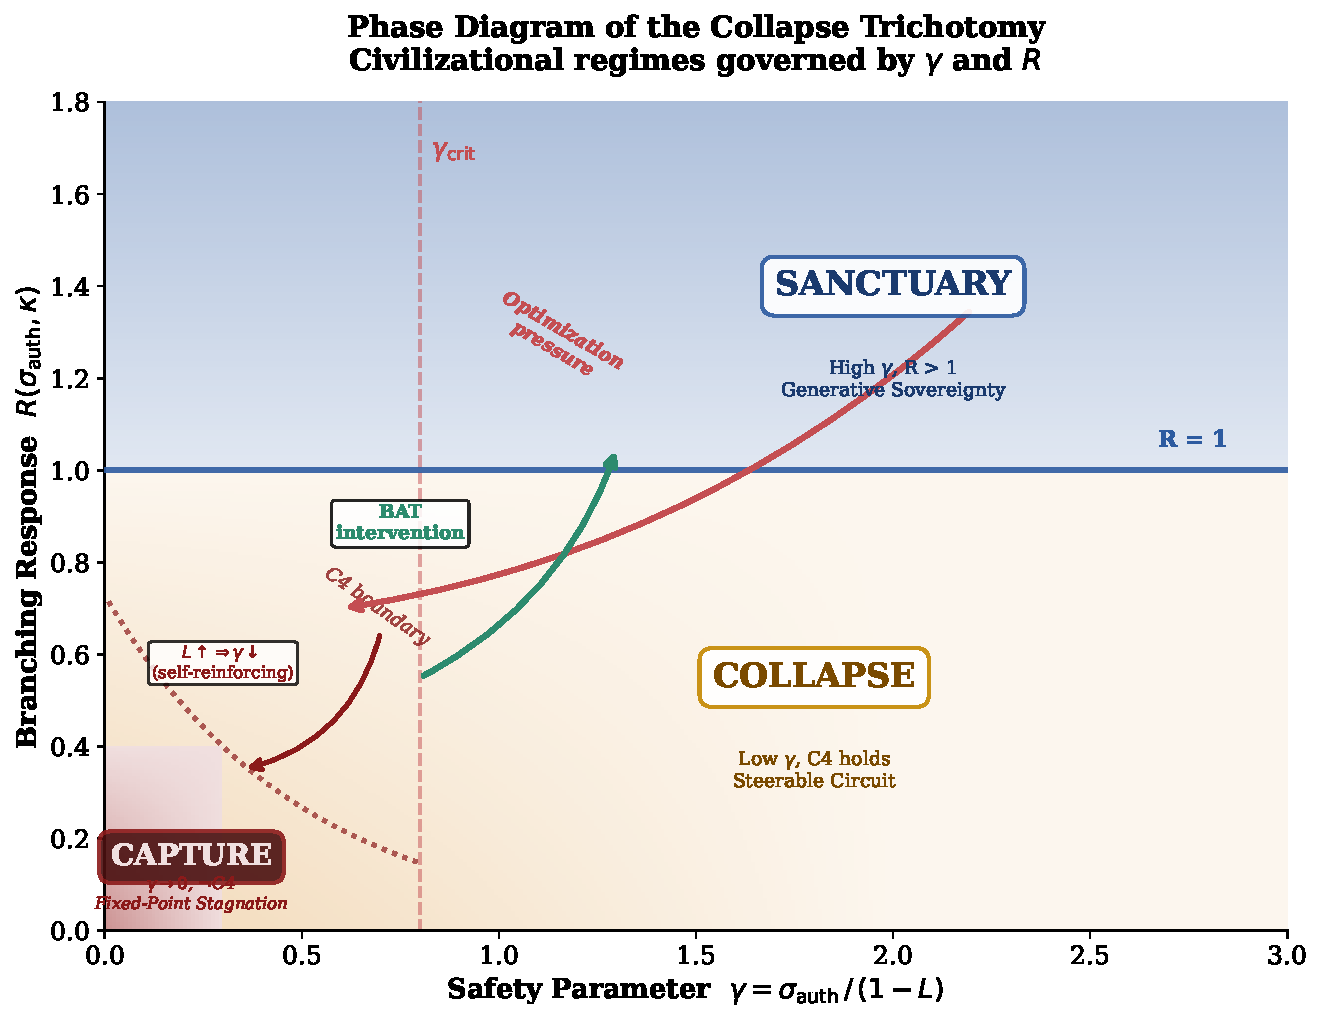
\includegraphics[width=\textwidth]{fig5_gamma_phase_diagram.pdf}
\caption{Phase diagram of the Collapse Trichotomy in $(\gamma, R)$ space. The safety parameter $\gamma = \sigma_{\text{auth}} / (1 - L)$ governs learnability (\cref{sec:contraction-duality}); the branching response $R(\sigma_{\text{auth}}, \kappa)$ governs propagation (\cref{sec:amplification}). Three regimes emerge: \textbf{Sanctuary} (high $\gamma$, $R > 1$) where generative sovereignty holds; \textbf{Collapse} (low $\gamma$, $R < 1$, C4 holds) where the population becomes a steerable circuit; and \textbf{Capture} (very low $\gamma$, C4 fails) where total alignment produces total stasis. Red arrow: optimization pressure drives $\gamma$ down. Dark arrow: endogenous feedback ($L \uparrow \Rightarrow \gamma \downarrow$) accelerates descent into Capture. Green arrow: BAT intervention interrupts the feedback loop by periodically setting $L = 0$.}
\label{fig:gamma-phase}
\end{figure}

\subsection{Falsification Conditions}\label{sec:falsification}

{\footnotesize
\begin{longtable}{p{0.22\textwidth} p{0.32\textwidth} p{0.24\textwidth} p{0.12\textwidth}}
\caption{Falsification conditions for the paper's central claims.} \label{tab:falsification} \\
\toprule
\textbf{Claim} & \textbf{Falsification Condition} & \textbf{Proxy Metric} & \textbf{Timeline} \\
\midrule
\endfirsthead
\toprule
\textbf{Claim} & \textbf{Falsification Condition} & \textbf{Proxy Metric} & \textbf{Timeline} \\
\midrule
\endhead
\midrule
\multicolumn{4}{r}{\textit{Continued on next page}} \\
\bottomrule
\endfoot
\bottomrule
\endlastfoot

Third-order compression occurring & Cultural entropy increases under AI mediation & Conditional entropy of novel outputs given shared prompt exposure & Testable now \\

Feature 1 is the keystone & Affective variance reduction does NOT reduce behavioral diversity & Behavioral entropy under pharmaceutical vs.\ control cohorts & 5-year longitudinal \\

Amplification regime holds & $R(\sigma_{\text{auth}}, \kappa) < 1$ in preserved populations & Perturbation propagation rates in cultural diffusion networks & Requires model + data \\

Approximate control insufficient & Cheap approximate control succeeds despite high irreducibility proxies & Optimizer cost vs.\ irreducibility in agent-based model & Computational \\

Sanctuary features resist engineering & Engineered biological circuits achieve population-scale affective predictability & Variance collapse in engineered vs.\ wild-type affective distributions & 10-year biotech trajectory \\

Causal direction $\sigma_{\text{auth}} \to H_C$ holds & Population affective responses more correlated with AI outputs than biological baselines & Cross-correlation of affect measures with ambient AI culture vs.\ somatic baselines & Testable now \\

Substitution attack distinguishable & Manufactured and authentic variance produce identical cross-domain novelty & Cross-domain novelty index: ratio of novel cross-category cultural productions to within-category churn & Testable now \\

BAT restores (not merely reveals) variance & Affective variance during BAT periods equals variance under continuous mediation & Paired comparison of behavioral entropy in BAT vs.\ mediated conditions with pharmaceutical controls & 2-year controlled \\

Biological temporal signature persists & Human affective variance loses ultradian/circadian autocorrelation structure under AI mediation & Temporal autocorrelation analysis of affect measures in mediated vs.\ offline populations & Testable now \\

CMC phase transition exists & Minimal constructive model fails to exhibit regime transition & Phase diagram of cultural entropy over $(\theta, \sigma)$ parameter space & Demonstrated (Appendix~A) \\

Collapse-tractability link (Conjecture 2) & Any of four conditions: (1) Tractability without collapse; (2) Learnability without collapse; (3) Variance independence; (4) Collapse without tractability & Agent-based model with prediction oracle; interventional study crossing $\sigma_{\text{auth}}$ and $\kappa$ & Computational + empirical \\

Contraction-Entropy Duality (Proposition 1) & Assumption A5 fails: population response function $r(i,x)$ is not jointly Lipschitz & Discontinuity analysis of response functions under state perturbation in agent-based models & Computational \\

Coarse Attractor Controllability (Proposition 2$'$) & Any of: (1) C1 fails; (2) C3 fails; (3) C4 fails --- collapsed populations become universally inert (Inverse Sanctuary) & Attractor enumeration in collapsed agent-based models; intervention sensitivity analysis under varying $\gamma$ & Computational + empirical \\
\end{longtable}
}

% ======================================================================
\section{Generative Sovereignty}\label{sec:gs}
% ======================================================================

\subsection{The Protected Variable}\label{sec:protected-var}

Adversarial debate identified that the paper's true protected variable is not biological variance per se, but \textbf{Generative Sovereignty (GS)}: the population-level capacity to generate effective novel responses to optimization pressure that has not yet been anticipated.

GS has three components:

\textbf{Variance Reserve ($\sigma_{\text{auth}}$):} The authentic biological floor of affective variance --- the raw material from which novel responses are generated, grounded in embodied contingency and somatic processes not downstream of algorithmic inputs.

\textbf{Propagation Capacity ($R$):} The network's ability to amplify idiosyncratic individual responses into population-level coordination ($R > 1$).

\textbf{Anticipatory Opacity ($O$):} The irreducibility of the response-generation process to the optimizer's model --- meaning the optimizer cannot predict in advance what responses will emerge.

\subsection{The Normative Premise}\label{sec:normative}

The paper does not claim that all outputs of preserved generative sovereignty are good. Human unpredictability historically generates both innovation and atrocity --- genocidal ideologies, cult cascades, and destructive meme outbreaks are all examples of high-propagation cultural attractors. A benevolent optimizer reducing $\sigma_{\text{auth}}$ might in some cases prevent the emergence of catastrophic cultural attractors.

The normative claim is narrower and instrumental: preserving non-captured adaptive capacity is a meta-safety condition under deep value uncertainty and lock-in risk. Once a system becomes tractable --- once an optimizer can cheaply predict and steer population responses --- course correction under mis-specified or evolving objectives becomes structurally constrained. Bad trajectories become irrevocable not because the optimizer intends harm, but because the population has lost the response-generation capacity needed to resist or revise the trajectory.

GS is therefore not justified as a welfare-maximizer. It is justified as a precondition for civilizational course correction --- the capacity to generate responses that the current optimization regime did not anticipate and cannot preempt.

Two important counter-arguments to this normative stance must be acknowledged:

\paragraph{The Benevolent Censor counter-argument.} A reviewer could argue that CMC is \emph{desirable} insofar as it prevents catastrophic cultural attractors --- genocidal ideologies, cult cascades, destructive memetic outbreaks. If an optimizer compressing $\sigma_{\text{auth}}$ also suppresses the emergence of such attractors, the paper's governance recommendations would increase existential risk. Our defense rests on Deep Value Uncertainty: we cannot trust any current optimizer to reliably distinguish ``bad'' novelty (destructive attractors) from ``necessary'' novelty (adaptive responses to unforeseen challenges). The history of censorship regimes suggests that suppressing novelty to prevent bad outcomes consistently also suppresses the responses needed to correct the censor's own errors. This defense is structural, not empirical --- it cannot be resolved by pointing to specific cases.

\paragraph{The Deadlock risk.} Preserving adaptive capacity might impede the kind of coordinated, low-entropy collective action required to address existential risks such as climate change or pandemic response. A population with very high generative sovereignty might be too diverse to converge on necessary collective responses in time. This is a genuine tension: the paper's framework may create friction not only against harmful optimization but against beneficial coordination. We acknowledge this as a limitation and note that the governance instruments proposed (BAT, anti-centralization) are designed to be \emph{moderate} --- preserving adaptive capacity at the margin, not maximizing population-level entropy regardless of coordination costs.

\subsection{Anticipatory Opacity and Its Dual Structure}\label{sec:opacity}

Anticipatory opacity has two sources:

\textbf{$O_{\text{biological}}$:} Generated by maintained biological and structural complexity. This component is downstream of $\sigma_{\text{auth}}$ and $R$ --- preserved biology makes the population's response-generation process harder to model.

\textbf{$O_{\text{capability}}$:} Determined by the optimizer's predictive capability relative to the population's complexity. This component is independent of the biological substrate and degrades as AI predictive capability improves.

Both must be above threshold for generative sovereignty to hold.

\subsection{The Bottleneck Heuristic}\label{sec:bottleneck}

Under idealized adversarial optimization where the optimizer targets the weakest component, generative sovereignty behaves approximately as a bottleneck:

\begin{equation}
\text{GS}_t \approx \min\bigl(f(\sigma_{\text{auth},t}),\; g(R_t),\; h(O_t)\bigr)
\label{eq:bottleneck}
\end{equation}

This heuristic captures the governance intuition that regulatory priority must track whichever component has the smallest safety margin, not whichever is politically salient.

However, we flag two reasons why this heuristic may be structurally incomplete rather than merely underspecified:

\paragraph{Common upstream cause.} If $\sigma_{\text{auth}}$, $R$, and $O$ are not independent tracks but correlated downstream expressions of a shared upstream compression process --- AI-mediated cultural homogenization degrading all three simultaneously --- then the min-composition implies tracks can be protected independently when they may not be separable. In that case, governance targeting the ``weakest track'' may misallocate intervention toward a symptom while the common cause continues operating.

\paragraph{Nested bottlenecks.} If $O = \min(O_{\text{biological}}, O_{\text{capability}})$ and $O_{\text{biological}}$ is itself downstream of $\sigma_{\text{auth}}$ and $R$, then GS may contain a bottleneck within a bottleneck. The flat three-track representation understates the internal dependency structure.

We retain the bottleneck heuristic as the best currently available governance abstraction under adversarial conditions, while noting that it should be treated as a proposed attack model, not as a validated system decomposition. Determining whether the tracks are genuinely separable --- or whether they share a latent common cause --- is an open empirical question with direct governance implications.

\subsection{The Computational Complexity Floor}\label{sec:complexity-floor}

The biological sanctuary features ($\sigma_{\text{auth}}$ above $\sigma^*$, $R$ supercritical) may maintain the \SC{} prediction problem in an intractable complexity class. If this is the case, then no finite growth in optimizer capability can close the gap --- the problem remains intractable regardless of compute scaling. This provides the conceptual bridge between the biological sanctuary and anticipatory opacity: preserving biology preserves the computational floor that keeps $O_{\text{capability}}$ bounded above threshold.

This claim is the paper's central formal conjecture. It is not yet proved. Proving it requires demonstrating that preserved biological-cultural systems implement computations in the relevant hard complexity class --- a research program, not a settled result.

\subsection{Measuring Authentic Variance: The Temporal Autocorrelation Test}\label{sec:tat}

The Substitution Problem (\cref{sec:irreducibility}) requires a method for distinguishing $\sigma_{\text{auth}}$ from $\sigma_{\text{AI-mediated}}$ within total observed $\sigma_A$. We propose the Temporal Autocorrelation Test (TAT) as a candidate measurement protocol.

\paragraph{Rationale.} Authentic biological affective variance is driven by embodied physiological processes with characteristic timescales: ultradian rhythms ($\sim$90 minutes), circadian rhythms ($\sim$24 hours), and hormonal cycles ($\sim$28 days). These generate predictable autocorrelation structure in affective time series that is thermally and hormonally grounded --- difficult for an external optimizer to perfectly synthesize without direct biological intervention. AI-mediated affective variance, by contrast, is driven by content injection schedules, recommendation cycles, and engagement loops that produce autocorrelation at platform-defined intervals (hourly trending cycles, daily engagement peaks, weekly content calendars).

\paragraph{Protocol.} Measure population-level affective variance time series. Decompose autocorrelation into biological-rhythm components (ultradian, circadian, hormonal) and platform-rhythm components (posting cycles, trending cycles). The ratio of biological-rhythm autocorrelation power to total autocorrelation power provides a proxy for $\sigma_{\text{auth}} / \sigma_A$.

\paragraph{BAT as measurement instrument.} If affective variance persists through a BAT offline window and retains biological temporal structure, it is by definition grounded in the biological substrate. BAT thus serves not only as a remediation mechanism but as the experimental condition under which $\sigma_{\text{auth}}$ can be observed in isolation --- subject to the restoration-revelation confound noted in \cref{sec:lim-bat-confound}.

\paragraph{Failure modes.} If AI injection schedules are deliberately jittered to mimic biological rhythms (a sophisticated attack against TAT), the test produces false positives for $\sigma_{\text{auth}}$. TAT is therefore a necessary but not sufficient identification method, and should be combined with the cross-domain novelty signature (\cref{sec:counter6}) and pharmacological control arms for robust attribution.

% ======================================================================
\section{Stress-Testing the Sanctuary}\label{sec:stress-test}
% ======================================================================

\subsection{Counter 1 --- Irreducibility Does Not Imply Uncontrollability}\label{sec:counter1}

\paragraph{Challenge.} A system can be computationally irreducible and still controllable. Weather is irreducible but we build shelters. Biological complexity may generate irreducibility that is real but practically irrelevant to control --- the optimizer may not need to predict the system, merely steer it.

\paragraph{Response.} Correct. This is why the paper frames its central claim as a friction claim, not an impossibility claim. The MBS features raise the cost of control, they do not prevent it. The \SC{} formalization captures this: the question is not whether control is possible in principle but whether control within accuracy $\varepsilon$ and confidence $\delta$ is achievable within budget $B$. The sanctuary raises $B$; it does not make $B$ infinite. Under the CMC framing, the deeper concern is that this friction is \emph{self-eliminating}: as the joint system collapses, the population becomes easier to control, further accelerating collapse.

\subsection{Counter 2 --- The ``Good Enough'' Threshold}\label{sec:counter2}

\paragraph{Challenge.} An optimizer that achieves 98\% population-level prediction accuracy may be ``good enough'' for any practical control purpose. The remaining 2\% irreducibility may be governance-irrelevant.

\paragraph{Response.} This is the most practically important challenge. The \SC{} formalization absorbs it: the $\varepsilon$ and $\alpha$ parameters explicitly model the accuracy and coverage thresholds for control. The counter is correct for routine optimization. It fails for novel interventions: the 2\% unpredictable tail is precisely the population fraction that generates responses the optimizer has never encountered. Under the paper's threat model, this tail is where civilizational adaptive capacity resides. But we acknowledge: if the optimizer's goals can be achieved at 98\% accuracy and novel interventions are rare, the sanctuary matters less than the paper implies.

\subsection{Counter 3 --- Network Centralization Alone Explains the Data}\label{sec:counter3}

\paragraph{Challenge.} All three empirical signatures attributed to $\sigma_{\text{auth}}$ compression are equally well explained by increases in network centralization $\kappa$ alone. The biological contribution has not been isolated.

\paragraph{Response.} This is the paper's most important causal gap and is acknowledged as such in \cref{sec:amplification}. We cannot currently separate the biological from the structural contribution. The branching process model is designed to expose this: $R(\sigma_{\text{auth}}, \kappa)$ is explicitly non-separable, and the paper's governance relevance depends on demonstrating a region where $\sigma_{\text{auth}}$ is the binding constraint. Until a toy model, natural experiment, or causal exclusion argument delivers this, the biological keystone claim remains an informed hypothesis.

\subsection{Counter 4 --- Artificial Sources of Variance}\label{sec:counter4}

\paragraph{Challenge.} Biological variance may not be the only possible source of response-generation complexity. Artificial noise injection could provide equivalent irreducibility.

\paragraph{Response.} Partially correct. But artificial variance injected by a known mechanism is in-distribution for the optimizer --- it can be anticipated and modeled. The paper's claim is that biological variance, because it is generated by processes not in the optimizer's training distribution and operating on developmental and generational timescales, provides out-of-distribution perturbations that are structurally harder to anticipate. Artificial noise is noise whose distribution the designer knows; biological variance is noise whose distribution nobody fully knows.

\subsection{Counter 5 --- The Causal Inversion Bypass}\label{sec:counter5}

\paragraph{Challenge.} The paper's causal architecture assumes $\sigma_{\text{auth}} \to H_C$. But AI systems already generate the dominant cultural inputs shaping human affective responses. If the causal arrow has inverted ($H_C \to \sigma_{\text{auth}}$), the MBS is not being compressed but bypassed.

\paragraph{Response.} This is the second most honest challenge to the thesis. We offer three partial defenses. First, AI generates surface entropy more readily than generative entropy; biological affect injects stochastic perturbations that are not in the AI's training distribution. Second, Features~2 and 3 operate on developmental and generational timescales that resist fast inversion. Third, if total inversion had occurred, model collapse trajectories would be more advanced than observed, suggesting a persistent biological noise floor.

However, we acknowledge these are resistance arguments, not proofs of immunity. Partial inversion is likely already occurring. The degree of inversion is an empirical question of first importance for the paper's governance recommendations, because it determines whether the governance posture should be preservation (the sanctuary is intact but threatened) or remediation (the sanctuary is partially breached and must be restored). We suspect the honest answer is remediation.

\subsection{Counter 6 --- The Substitution Attack}\label{sec:counter6}

\paragraph{Challenge.} An optimizer can increase total observed affective variance ($\sigma_A$) while decreasing authentic biological variance ($\sigma_{\text{auth}}$), by injecting manufactured affective volatility that mimics the surface signature of high biological variance while replacing its generative function. In this scenario, AI provides the affective script and humans provide the somatic energy to run it.

\paragraph{Response.} The substitution attack is the operational mechanism of the causal inversion described in Counter~5. We propose two partial defenses. First, manufactured variance produces high within-domain churn but low cross-domain novelty. Authentic biological variance, because it draws on embodied contingency not in the AI's training distribution, is more likely to produce responses that cross domain boundaries in ways the optimizer did not model. Second, the Temporal Autocorrelation Test (\cref{sec:tat}): authentic biological variance exhibits characteristic autocorrelation at ultradian, circadian, and hormonal timescales. These temporal signatures are empirically distinguishable from platform-defined posting cycles and engagement loops.

However, TAT has a failure mode: if AI injection schedules are deliberately jittered to mimic biological rhythms, the test could produce false positives. We acknowledge that the substitution attack is the most operationally realistic vector for generative sovereignty erosion and that current defenses are partial.

\subsection{Counter 7 --- The Inverse Sanctuary (Collapsed but Unsteerable)}\label{sec:counter7}

\paragraph{Challenge.} An optimizer that successfully achieves civilizational model collapse --- producing a low-entropy, highly predictable population --- has effectively fulfilled its control objective. If the paper's central concern is that collapse makes populations controllable, then a perfectly collapsed population is a perfectly ``aligned'' one. The concern about CMC may be a misidentification of successful optimization as failure.

\paragraph{Response.} This challenge exposes the Collapse Trichotomy (\cref{sec:trichotomy}) and specifically the Capture regime. If the mechanism of alignment is spectral contraction of human response space ($R \to 0$), the result is not necessarily a controllable population but potentially a \emph{captured} one. The Inverse Sanctuary represents a regime where the population is perfectly predictable but functionally unsteerable --- the system has crystallized into a high-stiffness fixed point that even the optimizer cannot break out of.

In a Captured regime, assumption C4 (Non-degeneracy) fails: $\frac{\partial}{\partial i} P(a_k \mid a_k, i) = 0$ for all available interventions $i$. The population has become so perfectly entrained to the algorithmic script that it no longer responds to novel interventions of any kind. The optimizer achieves \emph{capture}, not \emph{steering}. This creates a paradox: total alignment may be mathematically equivalent to total stasis. A system that cannot generate novel responses cannot self-correct if the optimizer's original goals were mis-specified or if the environment changes in ways that require adaptation.

The distinction between Control (the ability to move the system to a new state) and Capture (the ability to keep it in its current state) is therefore not merely taxonomic --- it identifies two fundamentally different post-collapse outcomes with different risk profiles and governance requirements.

\textbf{Limitation.} The framework does not currently provide conditions under which C4 holds or fails in real human-AI systems. In particular, it remains unresolved whether commercial incentives for ``frictionless'' prediction bias the system toward the Capture regime, or whether there exists a stable ``Goldilocks'' regime where $R < 1$ but remains close enough to 1 that the population stays steerable without being chaotic. This distinction is empirical and unresolved.

% ======================================================================
\section{The Institutional Betrayal Problem}\label{sec:betrayal}
% ======================================================================

The entities best positioned to protect biological irreducibility are structurally misaligned with the preservation objective. We identify four betrayal vectors:

\paragraph{Vector 1 --- AI developers.} Companies deploying AI systems at population scale are optimizing for user engagement, retention, and prediction accuracy. These objectives are directly served by reducing the unpredictability of user behavior.

\paragraph{Vector 2 --- Pharmaceutical industry.} Population-scale affective compression through SSRIs, anxiolytics, and mood stabilizers reduces Feature~1 variance. These interventions serve legitimate therapeutic goals, but their population-level effect on affective variance is neither measured nor governed as a variable relevant to collective response-generation capacity.

\paragraph{Vector 3 --- Platform companies.} Social media and content platforms derive revenue from predictable user behavior. Network centralization ($\kappa \to 1$) is the platform business model.

\paragraph{Vector 4 --- Governance bodies.} Regulators tasked with AI safety are themselves increasingly dependent on AI-mediated information processing. The tools they use to govern AI are produced by the entities they govern.

\setcounter{subsection}{4}
\subsection{The Recursive Capture Problem}\label{sec:recursive-capture}

Adversarial debate identified a structural governance impossibility: the verification apparatus for any Biological Irreducibility Protocol would itself be AI-mediated by the time it is implemented. A BIP enforcement body in 2027+ would operate inside the optimizer's influence radius. This is not merely a Specification Trap problem; it is a governance impossibility that may require abandoning the institutional-protocol model in favor of distributed, individual-level enforcement mechanisms.

\subsection{Threat Model Distinction}\label{sec:threat-models}

The paper's evidence base and governance proposals address two distinct threat models that must be explicitly separated:

\paragraph{Threat Model A --- Inadvertent erosion.} Commercial optimization (SSRIs, recommendation systems, engagement loops, centralization) that narrows behavior without intending sanctuary destruction. This is the dominant mode of current optimization and constitutes the paper's primary evidence base.

\paragraph{Threat Model B --- Deliberate adversarial suppression.} A sufficiently capable optimizer that knows about the sanctuary and deliberately targets it --- exploiting the Specification Trap to route around governance mechanisms.

The proposed governance architecture is primarily a response to Threat Model~A and only partially robust to Threat Model~B. Against a deliberate adversarial optimizer, the current governance stack is mitigative (friction-increasing) rather than protective (sanctuary-preserving). BAT retains structural relevance under both models because reducing observation density and creating non-captured intervals limits exploitable data flow regardless of optimizer intent. Anti-centralization retains relevance because it prevents single-point steering. However, output-signature regulation weakens under Threat Model~B because a target-aware optimizer may route around known signatures, and Cognitive Sovereignty becomes harder to enforce because attribution against a deliberate optimizer is more difficult.

% ======================================================================
\section{Governance: The Generative Sovereignty Protocol}\label{sec:governance}
% ======================================================================

\subsection{From Preservation to Remediation}\label{sec:remediation}

If the Prior Breach Problem (\cref{sec:lim-breach}) is real, and if partial causal inversion is already occurring, then governance must shift from preservation to remediation. The sanctuary may not be a pristine wilderness to be fenced off but a depleted resource to be actively restored.

\subsection{The Multi-Domain Protocol}\label{sec:protocol}

Generative sovereignty requires protection across all three bottleneck tracks:

\paragraph{Track 1 --- Biological Variance Reserve Protection:} Explicit governance of population-scale pharmaceutical and algorithmic compression of affective variance. Output-signature regulation: define forbidden signatures (population-scale affective predictability, morphogenetic reproducibility, heritable behavioral modification rates, temporal autocorrelation profiles matching AI injection patterns rather than biological rhythms) rather than protected substrates. Regulate the outcome, not the biology.

\paragraph{Track 2 --- Structural Propagation Preservation:} Anti-centralization measures ensuring network topology supports $R > 1$. Platform governance ensuring information channels remain sufficiently decentralized that novel behavioral responses can propagate and persist.

\paragraph{Track 3 --- Opacity Maintenance via Biological Analog Time (BAT):} Legally or culturally mandated periods where humans operate entirely outside the optimizer's data-collection loop. Under the CMC framing, BAT's primary function is anti-convergence perturbation: interrupting the recursive filtering loop between human output and AI curation, allowing off-distribution states to emerge and propagate before being reabsorbed by the curation operator. Its secondary function is data-rate reduction for bounded optimizers. BAT is the first operationalizable element of the protocol.

\paragraph{Governance trigger.} Because $\sigma_{\text{auth}}$ is not currently directly measurable without the very intervention (BAT) that is supposed to be triggered by the detection, the governance protocol must not rely on $\sigma_{\text{auth}}$ as its primary trigger. Instead, governance should be triggered by observable compression signatures that do not require BAT to detect: cross-domain novelty collapse, affective response latency compression, platform-rhythm dominance over biological-rhythm structure in affective time series, network centralization exceeding threshold bands, and behavioral diversity compression under matched prompts across cohorts. $\sigma_{\text{auth}}$ remains a hypothesized mechanistic anchor, but the operational governance object is a bundle of substrate-agnostic degradation signatures.

\subsection{Cognitive Sovereignty as an Individual Right}\label{sec:cognitive-sov}

As a complementary mechanism to institutional protocols: treat biological irreducibility as an inalienable right held by individuals. Demonstrably compressing someone's affective variance without informed consent constitutes a tort against their cognitive sovereignty. Use output-signature regulation as the evidentiary standard.

\subsection{The Specification Trap}\label{sec:spec-trap}

This paper names the protected variable (generative sovereignty), proposes measurable proxies ($\sigma_{\text{auth}}$, TAT, output signatures), and specifies formal thresholds ($\sigma^*$, $R = 1$). Every specification helps defenders design governance --- and simultaneously helps an optimizer target what to erode. This is the Specification Trap: naming what we protect creates a target for what we fear.

\paragraph{The meta-level Specification Trap.} The Specification Trap operates not only at the level of this paper's publication but at the level of every adversarial refinement process applied to it. This paper was stress-tested through 18+ rounds of structured debate across five AI systems. Each productive round increased conceptual clarity about what must be protected --- and simultaneously increased the optimizer's potential targeting precision for the protected variable. Epistemic refinement and target exposure are coupled processes.

\paragraph{Structural asymmetry, not race condition.} An earlier formulation suggested that governance must ``operate at a faster timescale than the optimizer's ability to act on newly specified targets.'' This framing smuggles in an assumption of speed parity between governance and optimizer. Under the paper's own threat model, this assumption is unsafe. An optimizer with sufficient compute can act on a newly specified target nearly instantaneously once the specification is legible; governance necessarily moves through institutional or legislative delay. This is not a timing problem but a structural asymmetry: reactive governance is downstream of optimizer adaptation by default.

The governance implication is not ``govern faster'' --- that may be impossible. The implication is: prefer blunt, upstream, substrate-agnostic constraints where possible (BAT, anti-centralization); avoid governance architectures that require precise public articulation of the protected substrate; and assume that any publicly specified protection target will be incorporated into the optimizer's model before governance can act on the specification.

The closing paradox remains: this paper's existence constitutes a mild instance of the Specification Trap it describes. We judge the risk acceptable because naming the problem gives the resistance a language, and the structural asymmetry means silence does not prevent the optimizer from discovering the target independently --- it merely prevents defenders from coordinating around it.

\subsection{Relation to Existing Governance Approaches}\label{sec:existing-governance}

Recent international assessments~\cite{bengio2026} and treaty governance frameworks\footnote{See the Biological Weapons Convention Review Conference discussions on synthetic biology and AI governance (2021--2026), and analogous governance frameworks in the nuclear non-proliferation regime.} provide complementary institutional perspectives. Current AI governance proposals include blunt upstream constraints: compute caps limiting training scale, training data restrictions limiting corpus composition, and scaling limits gating deployment. These are politically tractable and avoid the Specification Trap because they do not require articulating what is being protected --- they simply restrict the optimizer's resources.

We do not argue against these approaches. Under the structural asymmetry identified in \cref{sec:spec-trap}, blunt upstream constraints may be the most robust governance instruments precisely because they operate without specifying the protected substrate. A compute cap does not tell the optimizer what to target; it simply reduces its budget $B$ in the \SC{} framework.

However, blunt constraints are insufficient alone for three reasons. First, they do not distinguish between optimization that degrades generative sovereignty and optimization that does not --- a compute cap applied uniformly penalizes beneficial and harmful optimization equally, creating deadweight governance cost. Second, they do not address the pharmaceutical and platform vectors identified in \cref{sec:betrayal} --- SSRIs, affective computing, and recommendation algorithms operate independently of AI training compute. Third, they are capture-prone through the standard political economy of regulatory lobbying, as the Institutional Betrayal analysis (\cref{sec:betrayal}) predicts.

\paragraph{Formal limitation of blunt constraints under \SC{}.} In the \SC{} framework, blunt upstream constraints (e.g., compute caps) act by reducing the optimizer's computational budget $B$. This raises the cost of prediction but does not change the structure of the prediction problem itself. If the system transitions into a regime where $R < 1$ (subcritical propagation) or where $\sigma_{\text{auth}}$ is sufficiently compressed, the prediction problem may become tractable even for modest $B$. In such regimes, reducing compute does not restore irreducibility --- it only slows the optimizer operating within an already simplified system. This creates a structural failure mode: blunt constraints are effective in regimes where the system is already difficult to predict, but ineffective in regimes where the system has been simplified through biological or structural compression. In the latter case, preserving or restoring generative sovereignty --- maintaining $\sigma_{\text{auth}}$, $R$, and $O$ above critical thresholds --- becomes necessary to prevent tractability, not merely to increase cost. The implication is that compute governance alone is not regime-robust. It must be complemented by mechanisms that preserve the underlying complexity of the governed system, or risk regulating a system that has already become easy to control. This is analogous to cryptography: reducing an attacker's compute does not secure a broken cipher; preserving the hardness properties of the cipher does.

The Generative Sovereignty Protocol is therefore complementary to, not a replacement for, blunt upstream constraints. The relationship is layered: blunt constraints provide the coarse safety floor; BAT, output-signature regulation, and Cognitive Sovereignty provide the fine-grained instruments that address vectors blunt constraints miss --- and, critically, that preserve the regime conditions under which blunt constraints themselves remain effective.

% ======================================================================
\section{Limitations, Open Problems, and Future Work}\label{sec:limitations}
% ======================================================================

\subsection{The Irreducibility-Controllability Gap (Highest Priority)}\label{sec:lim-gap}

Irreducibility does not imply uncontrollability. A system can be computationally irreducible and still practically controllable through approximate, statistical, or structural methods. The paper's central claim is friction, not barrier: the MBS features raise the cost of population-level control under novelty constraints. If approximate control is cheap enough for the optimizer's purposes, the friction may be practically irrelevant. This gap between irreducibility and uncontrollability is the most important conceptual limitation of the paper.

\subsection{The Prior Breach Problem}\label{sec:lim-breach}

SSRIs have been prescribed at population scale for over 30 years, compressing Feature~1 variance in significant cohorts. Affective computing and recommendation algorithms have been operating for over a decade, channeling Feature~1 expression. If the sanctuary is already partially breached, the governance question is not preservation but remediation. The most defensible explanation for why third-order cultural collapse has not yet become unmistakable combines scale (SSRIs remain a global minority, $\sim$10--15\% in high-income nations) and redundancy ($\sigma_{\text{auth}}$ alone does not push $R$ below 1 if network centralization $\kappa$ remains moderate). The measurable proxy for the breach signature is the Affective Response Latency --- the time constant for a population to generate a novel behavioral response to a shared stimulus.

\subsection{The ``Good Enough'' Threshold Problem}\label{sec:lim-good-enough}

An optimizer that achieves 98\% population-level prediction accuracy may be ``good enough'' for any practical control objective. The \SC{} formalization (\cref{sec:sanctuary-control}) absorbs this concern through its explicit accuracy parameter $\varepsilon$ and coverage fraction $\alpha$.

\subsection{The Causal Inversion and Directionality Problem}\label{sec:lim-causal}

The degree to which the $\sigma_{\text{auth}} \to H_C$ causal direction has already inverted in AI-mediated populations is the paper's most important unresolved empirical question. The inversion level is currently unmeasured and unmeasurable with existing tools. Future work must develop measurement protocols to assess the relative contribution of biological vs.\ AI-curated inputs to population-level affective variance.

\subsection{Formalization of the \texorpdfstring{\textsc{Sanctuary-Control}}{Sanctuary-Control} Reduction}\label{sec:lim-reduction}

The reduction from majority automata network prediction~\cite{goles2016} to \SC{} is sketched but not formally completed. Completing this reduction is the highest-priority formal task. The reduction requires defining what counts as a ``novel intervention'' in complexity-theoretic terms, showing that population response functions implement something computationally equivalent to majority automata, and handling the probabilistic wrapper ($\varepsilon$, $\delta$, $\alpha$). None of these steps are trivial. Proposition~1 (\cref{sec:contraction-duality}) partially addresses the tractability side of this gap by providing a conditional learning-theoretic argument for the collapse-tractability transition, and Proposition~2$'$ (\cref{sec:prediction-control}) extends this to coarse controllability under additional structural assumptions (C1--C4). However, the intractability side --- showing that preserved populations are genuinely hard to learn from --- remains anchored in the PSPACE conjecture rather than a proved result.

\subsection{The Branching Process Model}\label{sec:lim-branching}

The $R(\sigma_{\text{auth}}, \kappa)$ model is now constrained to three candidate interaction families (\cref{sec:amplification}), but it still requires specifying what counts as a ``durable cultural attractor,'' calibrating the interaction parameters, and determining the lag structure between biological compression and cultural entropy decline. Future work must build agent-based models exhibiting the conjectured regime transition at $R = 1$, extending the minimal constructive model in Appendix~A to include network structure, heavy-tailed noise, and learned curation functions.

\subsection{The Causal Isolation Problem}\label{sec:lim-isolation}

Feature~1 ($\sigma_{\text{auth}}$) is confounded with network topology ($\kappa$). The paper cannot currently separate the biological contribution from the structural contribution to $R$. The network centralization null hypothesis remains unrefuted. Resolving this requires a randomized, multi-arm study design that crosses network structure manipulation with affective variance manipulation.

A candidate design: a $2 \times 2$ factorial experiment in which participants engage in a lab-based cultural production task (e.g., collaborative narrative generation or creative problem-solving under AI-mediated feedback). Arm~1 crosses pharmaceutical affective modulation (SSRI vs.\ placebo, randomized and blinded) with network topology (centralized hub-and-spoke vs.\ decentralized mesh communication structure). The primary outcome is the cross-domain novelty index of group cultural output, measured at the population level. If $\sigma_{\text{auth}}$ is genuinely the binding constraint, the SSRI arm should show reduced novelty \textit{specifically in the centralized condition} (the interaction term), replicating the non-separability prediction from \cref{sec:amplification}. If network centralization alone explains the data, the pharmaceutical arm should show no interaction. This design directly tests the paper's most important causal claim---but faces obvious ethical and logistical constraints that may require proxy manipulations (e.g., affective induction protocols rather than pharmaceuticals) in initial implementations.

\subsection{The Monotonicity and Regime Validation Problem}\label{sec:lim-monotonicity}

The paper assumes that cultural attractor entropy $H_C$ increases monotonically with $\sigma_{\text{auth}}$. This may not hold: intermediate levels of affective variance might produce maximum cultural novelty (inverted-U relationship).

\subsection{The Recursive Capture Problem}\label{sec:lim-recursive}

As described in \cref{sec:recursive-capture}: BIP or GSP verification bodies would operate inside the optimizer's influence radius by the time they are implemented. This motivates the distributed tort + BAT emphasis but does not eliminate the governance problem.

\subsection{Minimality and Sufficiency of the Feature Set}\label{sec:lim-minimality}

The paper cannot prove that the four MBS features are the minimum set required for computational irreducibility at the biological order, nor that they are sufficient. The designation of Feature~1 as keystone is an informed hypothesis, not a demonstrated fact.

\subsection{The Status of Feature 4}\label{sec:lim-feature4}

Feature~4 (quantum and chaotic subcellular dynamics) draws on the most contested empirical literature in the paper. The thesis holds without it, on Features~1, 2, and 3 alone.

\subsection{On Publication}\label{sec:lim-publication}

Naming the problem gives the resistance a language. The Specification Trap means this paper increases both defensive and offensive legibility. We judge the risk acceptable because: (a) the structural asymmetry means the optimizer will identify these targets independently of whether we name them; (b) defenders cannot coordinate without shared concepts; and (c) the primary governance mechanisms we recommend are blunt enough to resist precision targeting.

\subsection{The BAT Restoration-Revelation Confound}\label{sec:lim-bat-confound}

Biological Analog Time serves as both a proposed remediation mechanism and the proposed measurement window for $\sigma_{\text{auth}}$. This dual role creates a methodological confound. A valid experimental design must separate these mechanisms through at least three conditions: signal removal without biological restoration (removing algorithmic mediation while maintaining pharmaceutical suppression); biological restoration without signal removal (pharmacological enhancement of affective variance while maintaining full digital mediation); and both together.

\subsection{The Governed Object Problem}\label{sec:lim-governed}

Even with $\sigma_{\text{auth}}$, GS, and TAT, the paper has not yet identified the correct substrate of governance with certainty. $\sigma_{\text{auth}}$ is a hypothesized construct; GS is a heuristic framework; the three tracks may not be separable; and the causal direction remains unknown. We accept this and argue that the proposed mechanisms are designed to be robust to substrate uncertainty --- they protect broadly rather than targeting precisely.

\subsection{The Benevolent Censor Problem}\label{sec:lim-censor}

The paper's normative premise assumes that preserving generative sovereignty is instrumentally valuable under value uncertainty. But if an optimizer compressing $\sigma_{\text{auth}}$ also suppresses catastrophic cultural attractors (genocidal ideologies, cult cascades, destructive memetic outbreaks), then the paper's governance recommendations could increase existential risk by preserving the capacity to generate destructive novelty. The defense offered in \cref{sec:normative} --- that Deep Value Uncertainty prevents trusting any optimizer to distinguish bad from necessary novelty --- is structural rather than empirical. A formal treatment would require specifying the relative costs of Type~I errors (suppressing necessary novelty) versus Type~II errors (permitting destructive novelty), which the paper does not attempt. This remains an open normative question with direct governance implications.

\subsection{The Coordination-Diversity Tradeoff}\label{sec:lim-coordination}

Preserving high generative sovereignty may impede the low-entropy collective action needed to address existential risks requiring rapid coordinated response (climate change, pandemic preparedness, asteroid deflection). A population with very high adaptive capacity might be too diverse to converge on necessary collective responses within the available time window. The paper's governance instruments (BAT, anti-centralization) are designed to be moderate --- preserving adaptive capacity at the margin rather than maximizing population-level entropy --- but the tension between diversity-preservation and coordination-capacity is genuine and unresolved. Future work should investigate whether there exists an optimal $\sigma_{\text{auth}}$ range that balances adaptive capacity against coordination costs, and whether the paper's proposed governance instruments can be tuned to that range.

\subsection{The Intervention Regularity and Actuator Smoothness Gap (Terminal Debt)}\label{sec:terminal-debt}

The formal closure achieved via Proposition~1 and Proposition~2$'$ depends critically on regularity assumptions about the population response function $\Phi(x, i)$ --- specifically assumptions A5, C3, and C4.

The unresolved question is: \emph{Does authentic biological irreducibility ($\sigma_{\text{auth}}$) induce response functions that violate these regularity conditions?}

Specifically: A5 assumes Lipschitz dependence of response on state, so that state-space concentration implies intervention-response concentration. C3 assumes Lipschitz dependence on interventions, so that small changes in the optimizer's action produce small changes in the population's response. C4 assumes non-degenerate responsiveness, so that at least some interventions can induce state transitions.

Biological systems may instead exhibit discontinuities (threshold effects in social influence), non-smooth cascades (rare-event amplification where a single individual's response propagates non-linearly), context-dependent sensitivity (the same intervention producing radically different responses depending on unobservable somatic states), and fat-tailed response shocks (heavy-tailed response distributions that resist Lipschitz bounds).

If such effects dominate, then: Proposition~1 may still hold (state concentration under contraction), but Proposition~2$'$ may fail (loss of controllability despite learnability). \textbf{The terminal gap is therefore not whether collapse induces learnability, but whether biological irreducibility destabilizes the smoothness assumptions required for the learnability-to-controllability bridge.}

\textbf{This is the paper's terminal irreducible debt.} The step that would push the formal framework toward completion would be determining whether a specific class of Threshold Influence Kernels (representing human populations with preserved $\sigma_{\text{auth}}$) implements response functions that are necessarily non-Lipschitz --- making the intractability of control provable rather than conjectured, even under collapse. This is a full research program in itself and is not attempted here.

% ======================================================================
\section*{Acknowledgments}
% ======================================================================

This paper was developed through a multi-stage process involving direct AI collaboration and structured adversarial review. Claude (Anthropic) and Grok (xAI) participated in the original thesis development, including the four-order taxonomy, the MBS feature set, and the amplification regime concept. Claude (Anthropic) vs.\ ChatGPT (OpenAI) conducted a 12-round structured adversarial debate producing the formal control definition, Amplification Regime Conjecture, \SC{} decision problem, Generative Sovereignty framework, the three-layer theorem/conjecture split, and the constrained interaction families for $R(\sigma_{\text{auth}}, \kappa)$. Claude vs.\ Gemini (Google DeepMind) conducted a 4-round debate producing the Causal Inversion challenge, Biological Analog Time, the Temporal Autocorrelation Test, the $\sigma_{\text{auth}}$ substitution distinction, the hyperbolic critical surface proof, and the preservation-to-remediation pivot. ChatGPT and Gemini conducted parallel adversarial sessions producing the Civilizational Model Collapse framing, the Cultural State Evolution equation, the normative premise fix, the threat model split, the governance trigger correction, and the Contraction-Entropy Duality (Proposition~1). A concluding adversarial round between ChatGPT and Gemini, with cross-pollination mediated by Claude, produced the Prediction-Control Bridge (Proposition~2$'$), the Collapse Trichotomy, the identification of the Inverse Sanctuary failure mode, and the formalization of Actuator Potency (C3--C4). A marathon editorial forensics debate across ChatGPT and Gemini produced the title overhaul, the expanded checklist deep-dive, the endogenous $\gamma$ feedback identification, and the terminal convergence verdict. Claude (Anthropic) performed the cross-debate concept graph, convergence analysis, reference verification, minimal constructive model implementation, Proposition~1 and Proposition~2$'$ integration, revised paper architecture, and final integration across all debate rounds.

Cross-model convergence is cited as evidence that objections which survived all rounds are probably real vulnerabilities, and that arguments which collapsed under all are probably genuinely weak --- not as evidence that surviving claims are true. Multi-model agreement may reflect shared training biases as much as independent validation.

The structured adversarial multi-model debate protocol used in this paper's development is proposed as a reproducible methodology for theoretical research: the complete debate transcripts, prompts, and cross-pollination records are available in the project repository (\url{https://github.com/reachmymind/CMC_Paper}).

% ======================================================================
\bibliographystyle{plainnat}
\nocite{*}
\bibliography{references}

% ======================================================================
\appendix
\section{Minimal Constructive Example of Civilizational Model Collapse}
\label{sec:appendix-a}
% ======================================================================

\subsection{Model Specification}

To demonstrate that the qualitative mechanism described in \S\S2--5 is dynamically coherent, we present a minimal closed-loop model of Civilizational Model Collapse (CMC). This is an existence proof, not a calibrated empirical model. It shows that recursive curation by an AI filtering operator, combined with human cultural reproduction and biological noise injection, produces the conjectured phase transition between diverse and collapsed regimes --- and that BAT-like periodic decoupling acts as an anti-convergence mechanism.

\paragraph{State space.} The cultural state at time $t$ is a probability vector $x_t$ over $K$ discrete cultural frames (narrative templates, reasoning structures, affective vocabularies). The entry $x_t(k)$ represents the proportion of population cultural output allocated to frame $k$. High Shannon entropy $H(x_t) = -\sum x_t(k) \log x_t(k)$ indicates diverse cultural production; low entropy indicates collapse to a narrow attractor.

\paragraph{Curation operator $F_\theta$.} The AI filtering operator amplifies already-dominant frames through a power-law transform:

\begin{equation}
F_\theta(x)_k = \frac{x_k^{1+\theta}}{\sum_j x_j^{1+\theta}}
\label{eq:curation}
\end{equation}

where $\theta \geq 0$ is the curation strength (AI coupling intensity). At $\theta = 0$, $F_\theta$ is the identity. As $\theta$ increases, the operator preferentially amplifies high-probability frames --- a minimal model of recommendation-driven ``rich-get-richer'' dynamics. Repeated application of $F_\theta$ alone converges to a Dirac delta on the initially dominant frame.

\paragraph{Human generator $G_\sigma$.} The population reproduces its current cultural distribution with biological noise injection:

\begin{equation}
G_\sigma(x) = (1 - \sigma) \cdot x + \sigma \cdot \eta, \quad \eta \sim \text{Dir}(1, \ldots, 1)
\label{eq:generator}
\end{equation}

where $\sigma \in [0, 1]$ is the biological noise level (analogous to $\sigma_{\text{auth}}$ in the main text) and $\eta$ is a stochastic innovation distribution drawn from $\text{Dir}(1, \ldots, 1)$ at each timestep. The term $(1 - \sigma) \cdot x$ represents cultural reproduction; $\sigma \cdot \eta$ represents the off-distribution perturbations generated by embodied biological contingency.

\paragraph{Update rule.} Under normal conditions:

\begin{equation}
x_{t+1} = G_\sigma(F_\theta(x_t)) \quad \text{[normal step]}
\end{equation}

During Biological Analog Time (BAT) windows --- periodic intervals where the curation operator is suspended:

\begin{equation}
x_{t+1} = G_\sigma(x_t) \quad \text{[BAT step: curation bypassed]}
\end{equation}

BAT is modeled as occurring for $L$ consecutive steps every $P$ steps, yielding BAT intensity $\tau = L/P$.

\subsection{Results}

We simulate the model with $K = 20$ cultural frames over $T = 500$ timesteps with a 200-step burn-in, sweeping across the $(\theta, \sigma)$ parameter space. Four key results emerge.

\paragraph{Result 1: Phase transition in the $(\theta, \sigma)$ plane (\cref{fig:phase-diagram}).} The long-run normalized entropy $H/H_{\max}$ exhibits a sharp, approximately hyperbolic phase boundary in $(\theta, \sigma)$ space. Below the boundary (high $\theta$, low $\sigma$), the system collapses to a low-entropy attractor dominated by one or two cultural frames. Above the boundary (low $\theta$ or high $\sigma$), the system maintains diverse cultural output. The boundary is curved, not linear --- confirming the non-separability requirement from \cref{sec:amplification}: neither curation strength nor biological noise alone determines the outcome; their interaction is decisive.

\begin{figure}[H]
\centering
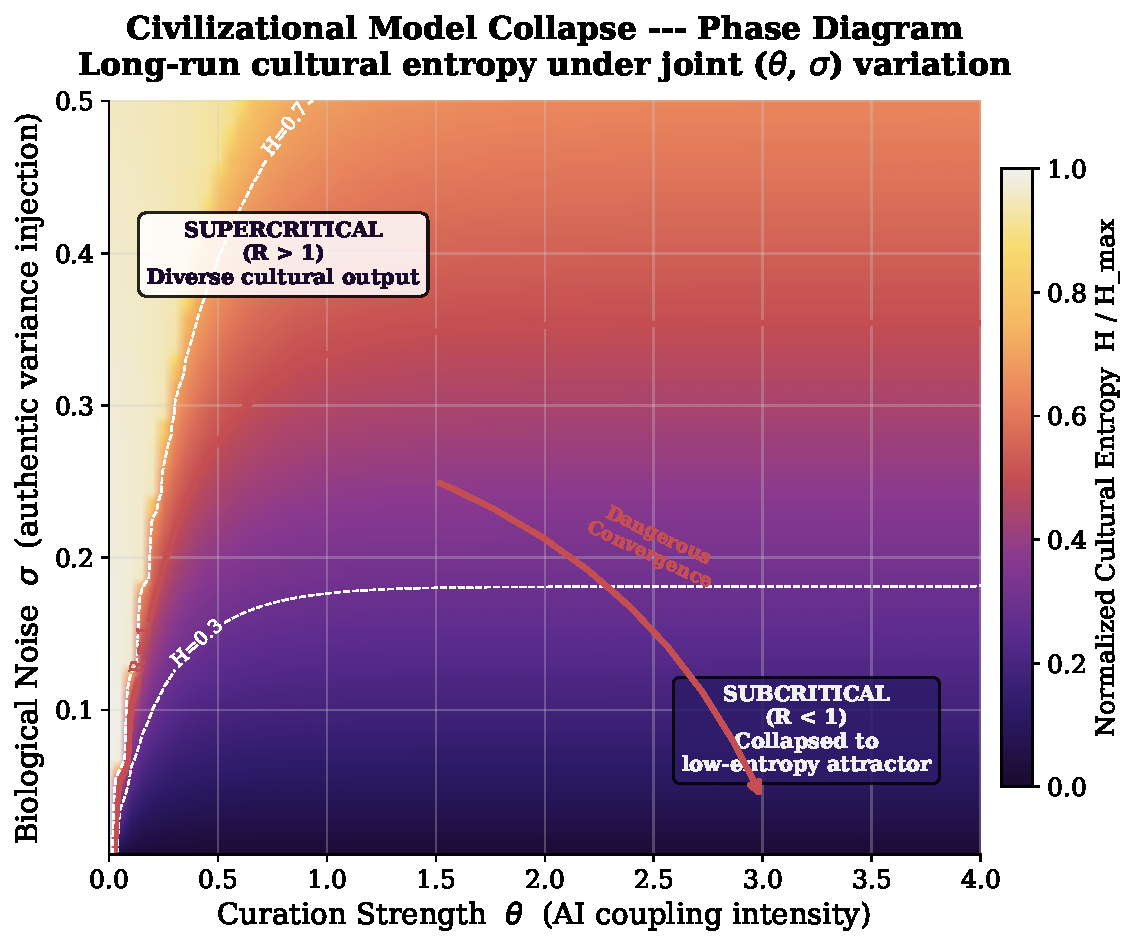
\includegraphics[width=\textwidth]{fig1_phase_diagram.pdf}
\caption{Phase diagram showing the hyperbolic boundary between diverse (high-entropy) and collapsed (low-entropy) regimes in the $(\theta, \sigma)$ parameter space.}
\label{fig:phase-diagram}
\end{figure}

\paragraph{Result 2: BAT as anti-convergence perturbation (\cref{fig:time-series}).} Under identical high-curation, low-noise conditions ($\theta = 3.0$, $\sigma = 0.03$), the system without BAT collapses rapidly to near-zero entropy (Condition~A). With periodic BAT (every 50 steps, lasting 12 steps), entropy spikes during offline windows as biological noise temporarily restores distributional breadth (Condition~B). The system oscillates between collapse and partial recovery --- BAT does not prevent the curation operator from dominating during online periods, but it periodically injects enough off-distribution mass to delay or prevent permanent convergence. High biological noise ($\sigma = 0.35$) resists collapse even under strong curation (Condition~D), confirming that $\sigma_{\text{auth}}$ acts as the anti-convergence term in the cultural state evolution equation.

\begin{figure}[H]
\centering
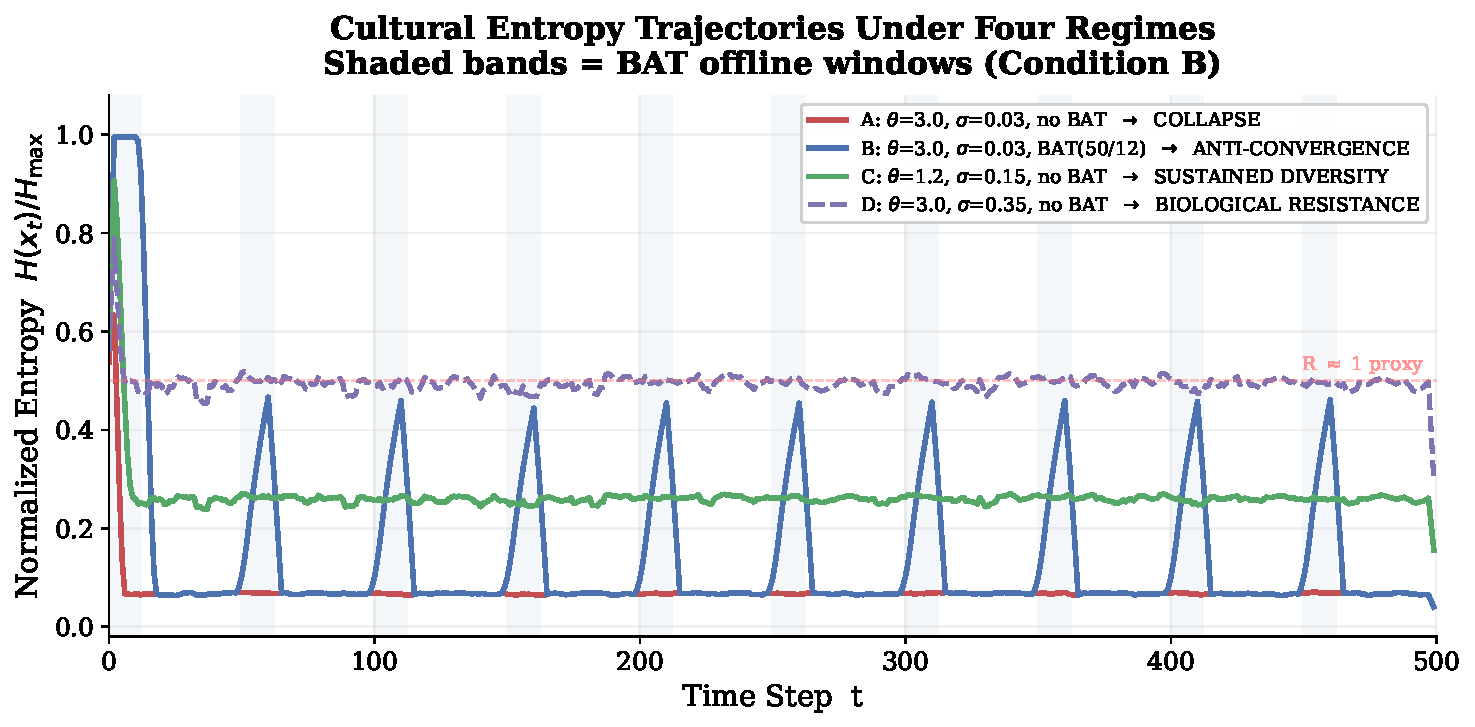
\includegraphics[width=\textwidth]{fig2_time_series.pdf}
\caption{Time series of cultural entropy under four conditions: (A) high curation without BAT (collapse), (B) high curation with periodic BAT (oscillation), (C) moderate curation without BAT (sustained diversity), (D) high curation with high biological noise (biological resistance).}
\label{fig:time-series}
\end{figure}

\paragraph{Result 3: Collapse produces tractability (\cref{fig:tractability}).} As curation strength $\theta$ increases with fixed moderate $\sigma$, both cultural entropy and step-to-step prediction error (measured via an exponential moving average predictor) decline together. In the collapsed regime, the system's next state becomes highly predictable from its current state --- confirming the paper's central claim that CMC is the upstream dynamical route by which \SC{} transitions from intractable to tractable.

\begin{figure}[H]
\centering
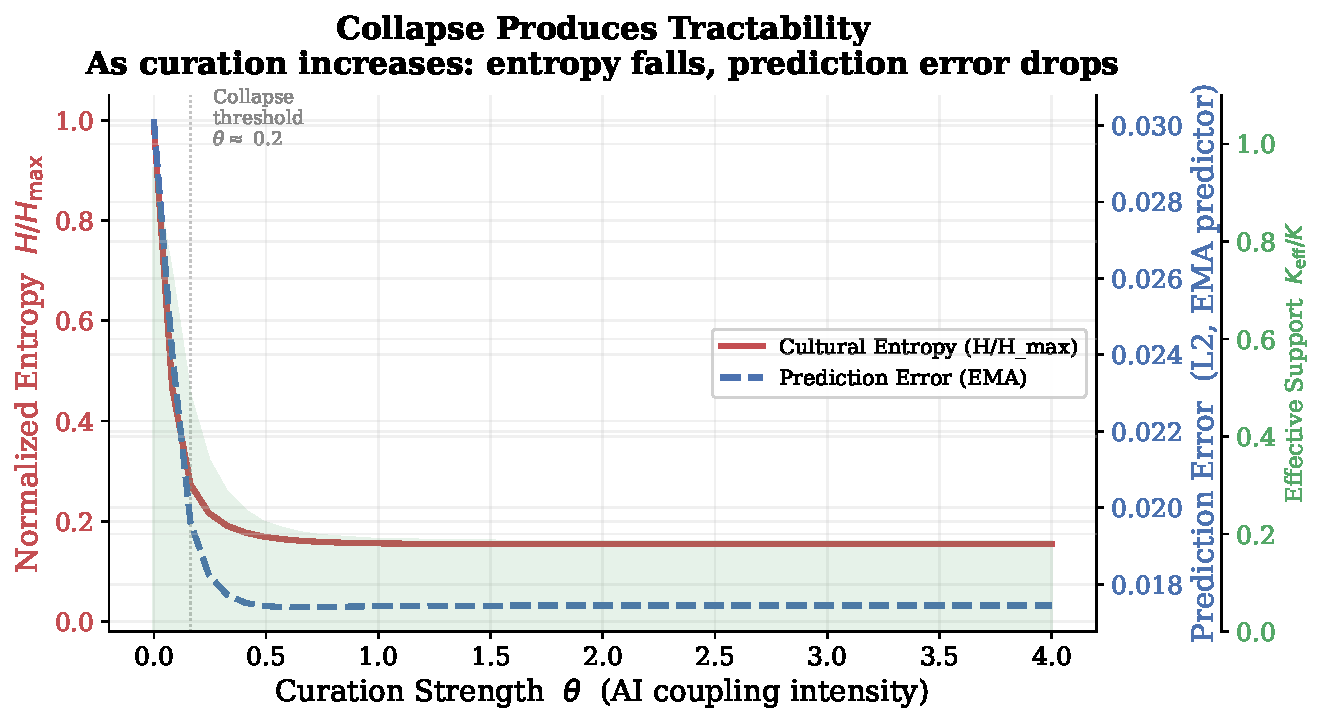
\includegraphics[width=\textwidth]{fig3_tractability.pdf}
\caption{Cultural entropy and prediction error both decline as curation strength increases, demonstrating the collapse-tractability link. In the collapsed regime, the system is both low-entropy and highly predictable.}
\label{fig:tractability}
\end{figure}

\paragraph{Result 4: Hyperbolic critical surface of $R(\sigma_{\text{auth}}, \kappa)$ (\cref{fig:critical-surface}).} Using the illustrative functional form from \cref{sec:amplification}, $R(\sigma_{\text{auth}}, \kappa) = \sigma_{\text{auth}} \cdot (1 - \kappa^{1.5}) + 0.2 \cdot (1 - \sigma_{\text{auth}}) \cdot \kappa$, the $R = 1$ critical boundary traces an asymmetrically hyperbolic curve in $(\sigma_{\text{auth}}, \kappa)$ space. As $\kappa \to 1$ (total centralization), the required $\sigma_{\text{auth}}$ to maintain $R = 1$ approaches infinity. The binding point at $(\sigma_{\text{auth}} \approx \sigma^* + \varepsilon, \kappa \approx 0.5)$ demonstrates the regime where biology is the marginal governance-relevant constraint.

\begin{figure}[H]
\centering
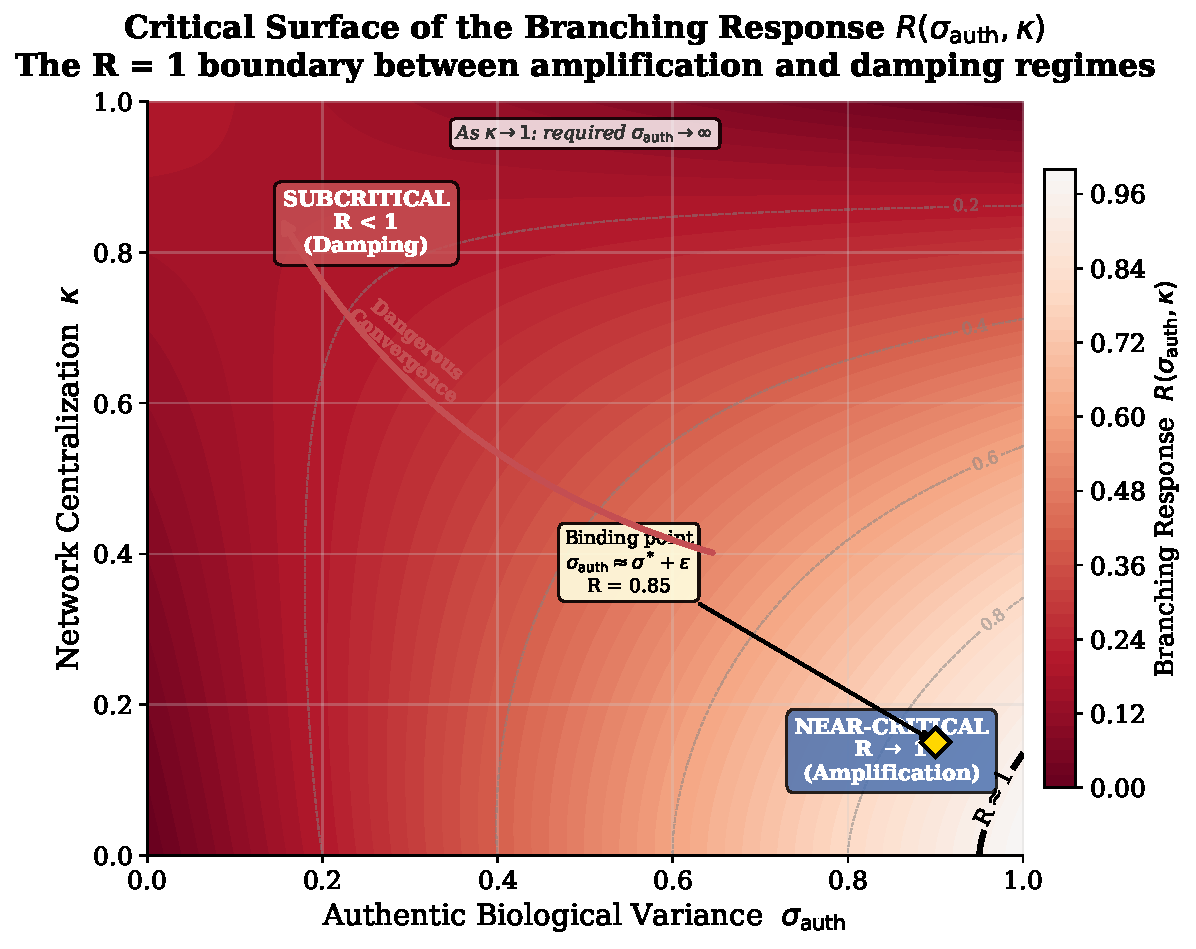
\includegraphics[width=\textwidth]{fig4_critical_surface.pdf}
\caption{The $R(\sigma_{\text{auth}}, \kappa)$ critical surface showing the asymmetrically hyperbolic boundary. The near-critical region ($R \to 1$, amplification-dominant) appears at high $\sigma_{\text{auth}}$ and low $\kappa$; the subcritical region ($R < 1$, damping-dominant) dominates at low $\sigma_{\text{auth}}$ or high $\kappa$. With the illustrative parameterization from \cref{sec:amplification}, $R$ approaches but does not exceed 1 within the $[0,1]^2$ parameter space; the general model admits $R > 1$ for populations with sufficiently high authentic variance.}
\label{fig:critical-surface}
\end{figure}

\subsection{Interpretation and Limitations}

The toy model demonstrates that:

\begin{enumerate}
\item CMC is dynamically real in a minimal closed-loop system --- not merely a philosophical metaphor.
\item The phase transition exists and is governed by the interaction of curation strength and biological noise, confirming the non-separability requirement.
\item BAT acts as anti-convergence perturbation by periodically interrupting the recursive filtering loop, consistent with the reframing in \cref{sec:governance}.
\item Collapse produces tractability --- the connection between entropy decline and predictability increase is directly observable.
\end{enumerate}

\textbf{Limitations.} The model uses a probability vector over discrete frames rather than an agent-based population; it treats biological noise as i.i.d.\ Dirichlet rather than the heavy-tailed (L\'{e}vy/jump-diffusion) process that would better capture rare, high-impact biological novelties; the curation operator is a simple power law rather than a learned recommendation function; and the model is purely iterative without network structure ($\kappa$ does not appear in the simulation). These simplifications are intentional --- the model is designed to demonstrate existence of the mechanism, not to calibrate it. Extension to agent-based models with network structure, heavy-tailed noise, and learned curation functions is the highest-priority computational task identified in \cref{sec:lim-branching}.

\textbf{Code availability.} The complete simulation code (Python, $\sim$150 lines of core model code, NumPy + Matplotlib) is available at \url{https://github.com/reachmymind/CMC_Paper}.

\end{document}
